
\documentclass{llncs}  

\usepackage{amsfonts}
\usepackage{amssymb,amsmath}
\usepackage{graphicx}
\usepackage[english]{babel}
\usepackage{listings}
\usepackage{hyperref}
\usepackage[utf8]{inputenc} 
\usepackage{latexsym}
\usepackage{eurosym}
\usepackage{array}
\usepackage{timestamp}
\usepackage{epstopdf}
\usepackage{multicol}
\usepackage{multirow}
\usepackage{lscape}


%\usepackage[pagewise]{lineno}



%\def\thepage{\arabic{page}--[\timestamp]} 
\usepackage{tikz}
\usetikzlibrary{snakes}

%\setcounter{tocdepth}{5}

% $Id: macros.tex,v 1.8 2012/07/19 22:21:36 ccamacho Exp $
% \newenvironment{definition}{\par\bf\bigskip \bigskip Definition}{\bigskip \bigskip}{\rmfamily}
% \newenvironment{example}{\par\bf\bigskip \bigskip Example}{\bigskip \bigskip}{\rmfamily}
% \newenvironment{lemma}{\par\bf\bigskip \bigskip  Lemma}{\bigskip \bigskip}{\rmfamily}
% \newenvironment{proof}{\par{\bf\bigskip \bigskip  Proof}}{\bigskip \bigskip}{\rmfamily}
% \newenvironment{proposition}{\par\bf \bigskip\bigskip  Proposition}{\bigskip \bigskip}{\rmfamily}
% \newenvironment{corollary}{\par\bf \bigskip\bigskip  Corollary}{\bigskip \bigskip}{\rmfamily}
% \newenvironment{theorem}{\par\bf \bigskip \bigskip Theorem}{\bigskip \bigskip}{\rmfamily}

%Fin de Carlos

% $Id: macros.tex,v 1.8 2012/07/19 22:21:36 ccamacho Exp $
\def\squareforqed{\hbox{\rlap{$\sqcap$}$\sqcup$}}

% Carlos
% He eliminado los cubos del qed, luego podemos mirar
% si queda algun simbolo mejor
\def\qed{
       \ifmmode\squareforqed\else{\unskip\nobreak\hfil
    \penalty50\hskip1em\null\nobreak\hfil\squareforqed
    \parfillskip=0pt\finalhyphendemerits=0\endgraf}\fi
}

%\usepackage{marginnote}
%\renewcommand{\marginfont}{\fontsize{6}{8}\selectfont}



\newcommand{\ccomens}[2]{\uwave{#1\ccomen{#2}}}
\def\lcomen#1{\footnote{\textbf{Comentario de Luis}: \textcolor{red}{#1}}}
\def\ccomen#1{\footnote{\textbf{Comentario de Carlos}: \textcolor{blue}{#1}}}
\def\acomen#1{\footnote{\textbf{Comentario de Alberto}: \textcolor{green}{#1}}}



\newcommand{\comment}[2]{\footnote{\textbf{#1}: #2}}

\newcommand{\ComaMat}{}
\newcommand{\PuntoMat}{}
%\newenvironment{proof}{Proof}


\newcommand{\ismcomment}[1]{}
\newcommand{\bdfn}{\begin{definition} \begin{rm}}
\newcommand{\edfn}{\end{rm}$ $\qed \end{definition}}

\newcommand{\bprf}{\begin{proof}}
\newcommand{\eprf}{\leavevmode\qed \end{proof}}

\newcommand{\bthm}{\begin{theorem} \begin{rm}}
\newcommand{\ethm}{\end{rm}$ $\qed \end{theorem}}

\newcommand{\bprop}{\begin{proposition} \begin{rm}}
\newcommand{\eprop}{\end{rm}$ $\qed  \end{proposition}}

\newcommand{\bcor}{\begin{corollary}\begin{rm}}
\newcommand{\ecor}{\end{rm}$ $\qed  \end{corollary}}

\newcommand{\blem}{\begin{lemma}\begin{rm}}
\newcommand{\elem}{\end{rm}$ $\qed  \end{lemma}}

\newcommand{\bfact}{\begin{fact}\begin{rm}}
\newcommand{\efact}{\end{rm}$ $\qed  \end{fact}}

\newcommand{\bex}{\begin{example}\begin{rm}}
\newcommand{\eex}{\end{rm}$ $\qed  \end{example}}

\newenvironment{defn}{\bdfn}{\edfn}
\newenvironment{proofappendix}[1]{\textbf{\emph{Proof of #1}}}{}
\newcommand{\barra}{\:| \:}
\def\y{\;\wedge\;}
\def\o{\;\vee\;}
\newcommand{\union}{\cup}
\newcommand{\contenido}{\subseteq}
\newcommand{\interseccion}{\cap}
\newcommand{\Vacio}{\emptyset}
\renewcommand{\emptyset}{\varnothing}

\newcommand{\true}{\mathtt{true}}
\newcommand{\false}{\mathtt{false}}
\newcommand{\entonces}{\mathtt{\ then\  }}
\newcommand{\sino}{\mathtt{\ else\  }}
\newcommand{\si}{\ \mathrm{if}\ }

\newcommand{\letbar}[1]{\mbox{I\kern-0.23em#1}}
\newcommand{\nat}{\letbar N}
\newcommand{\real}{\letbar R}
\newcommand{\realm}{\letbar R_+^m}
\newcommand{\Bool}{\texttt{Bool}}
%
\newcommand{\comen}[1]{
}
\newcommand{\timed}{{\mathtt{Time}}}
\newcommand{\outputs}[1]{\ensuremath{\mathtt{ outputs}(#1)}}
\newcommand{\representative}[2]{\ensuremath{\mathtt{ moreR}(#1,#2)}}
\newcommand{\msTOs}[1]{\ensuremath{\mathtt{ msTOs}(#1)}}
\newcommand{\setnttr}[2]{\ensuremath{\mathtt{ setnttr}(#1,#2)}}
\newcommand{\minTime}[1]{\ensuremath{\mathtt{ mT}(#1)}}
\newcommand{\maxTime}[1]{\ensuremath{\mathtt{ MT}(#1)}}
\newcommand{\minimo}[1]{\ensuremath{\mathtt{ min}\left\{\!#1 \!\!\!\!\right\}}}
\newcommand{\maximo}[1]{\ensuremath{\mathtt{ max}\left\{\!#1 \!\!\!\!\right\}}}
\newcommand{\FSM}{\texttt{FSM}}
\newcommand{\FSMs}{\texttt{FSMs}}
\newcommand{\EFSM}{\texttt{EFSM}}
\newcommand{\EFSMs}{\texttt{EFSMs}}
\newcommand{\TFSM}{\texttt{TFSM}}
\newcommand{\TFSMs}{\texttt{TFSMs}}
\newcommand{\TPEM}{\texttt{TPEM}}
\newcommand{\TPEMs}{\texttt{TPEMs}}

\newcommand{\SPLs}{\texttt{SPLs}}
\newcommand{\SPL}{\texttt{SPL}}
\newcommand{\PLs}{\texttt{PLs}}
\newcommand{\PL}{\texttt{PL}}
\newcommand{\FODAT}{\texttt{AT}}

\newcommand{\FODA}{\texttt{FODA}}
\newcommand{\fodaPA}{\ensuremath{\mathtt{fodaA}}}
\newcommand{\fodaPAp}{\ensuremath{\mathtt{SPLA{^\calP}}}}
\newcommand{\fodaPAbasic}{\ensuremath{\mathtt{fodaA_b}}}
\newcommand{\wellstructured}{\ensuremath{\mathtt{fodaA_{ws}}}}
\newcommand{\normalForm}{\ensuremath{\mathtt{fodaA_{nf}}}}
\newcommand{\prenormalForm}{\ensuremath{\mathtt{fodaA_{pre}}}}
\newcommand{\RSEB}{\texttt{RSEB}}
\newcommand{\PLUSS}{\texttt{PLUSS}}
\newcommand{\np}{\mathtt{np}}




 %

\newcommand{\afterCond}[1]{\texttt{afterCond}(#1)}
\newcommand{\afterInp}[1]{\texttt{afterInp}(#1)}
\newcommand{\IUT}{\texttt{IUT}}
%\newcommand{\case}{\texttt{Case :}}
\newcommand{\HOTL}{{\cal HOTL}}
\newcommand{\wc}{wild-card}

\newcommand{\calA}{{\cal A}}
\newcommand{\calB}{{\cal B}}
\newcommand{\calC}{{\cal C}}
\newcommand{\calD}{{\cal D}}
\newcommand{\calE}{{\cal E}}
\newcommand{\calF}{{\cal F}}
\newcommand{\calG}{{\cal G}}
\newcommand{\calH}{{\cal H}}
\newcommand{\calI}{{\cal I}}
\newcommand{\calL}{{\cal L}}
\newcommand{\calM}{{\cal M}}
\newcommand{\calN}{{\cal N}}
\newcommand{\calO}{{\cal O}}
\newcommand{\calP}{{\cal P}}
\newcommand{\calQ}{{\cal Q}}
\newcommand{\calR}{{\cal R}}
\newcommand{\calS}{{\cal S}}
\newcommand{\calT}{{\cal T}}
\newcommand{\calU}{{\cal U}}
\newcommand{\calV}{{\cal V}}
\newbox\arriba
\newbox\abajo
\newbox\CaracterInterno
\newbox\CaracterDerecha
\newdimen\anchura
\def\MacrosTranGeneral#1#2#3#4#5#6{%
  \setbox\CaracterInterno=\hbox{\mathsurround=0pt$\mathord#4$}
  \setbox\CaracterDerecha=\hbox{\mathsurround=0pt$\mathord#3$}
  \setbox\arriba=\hbox{$#1#2$}
  \setbox\abajo=\hbox{\mathsurround=0pt%
                      \anchura=\wd\arriba%
                      \advance \anchura by 0.5em%
                      \divide \anchura by \wd\CaracterInterno%
                      \multiply \anchura by \wd\CaracterInterno%
                      \copy\CaracterInterno\kern\SeparacionInternaFlecha
                      \hbox to \anchura{%
                          $\cleaders%
                            \hbox{\kern\SeparacionInternaFlecha\copy\CaracterInterno}
                            \hfill$}%
                      \kern\SeparacionExternaFlecha\copy\CaracterDerecha}
  \mathrel{{\buildrel\vbox{\copy\arriba \kern\SeparacionFlechaArriba} %
    \over{\copy\abajo^{#6}}}_{#5}}
  }
\def\MacrosTranGeneralProp#1#2#3#4#5{\mathchoice%
  {\MacrosTranGeneral{\scriptstyle}{#1}{#2}{#3}{#4}{#5}}
  {\MacrosTranGeneral{\scriptstyle}{#1}{#2}{#3}{#4}{#5}}
  {\MacrosTranGeneral{\scriptscriptstyle}{#1}{#2}{#3}{#4}{#5}}
  {\MacrosTranGeneral{\scriptscriptstyle}{#1}{#2}{#3}{#4}{#5}}}

\def\MacrosTran#1{%
  \def\SeparacionInternaFlecha{-0.3em}
  \def\SeparacionExternaFlecha{-0.5em}
  \def\SeparacionFlechaArriba{-3pt}
  \MacrosTranGeneralProp{#1}{\rightarrow}{-}{}{}}
\def\MacrosNoTran#1{%
  \def\SeparacionInternaFlecha{-0.3em}
  \def\SeparacionExternaFlecha{-0.5em}
  \def\SeparacionFlechaArriba{-3pt}
  \MacrosTranGeneralProp{#1\kern 0.5em}{{\not\rightarrow}}{-}{}{}}
\def\MacrosVTran#1{%
  \def\SeparacionInternaFlecha{-0.2em}
  \def\SeparacionExternaFlecha{-0.5em}
  \def\SeparacionFlechaArriba{0pt}
  \MacrosTranGeneralProp{#1}{\Rightarrow}{=}{}{}}
\def\MacrosNoVTran#1{%
  \def\SeparacionInternaFlecha{-0.2em}
  \def\SeparacionExternaFlecha{-0.5em}
  \def\SeparacionFlechaArriba{-3pt}
  \MacrosNoTranGeneralProp{#1}{\not\Rightarrow}{=}{}{}}
\def\tran#1{\ensuremath\mathbin{\MacrosTran{#1}}}
\def\vtran#1{\ensuremath\mathbin{\MacrosVTran{#1}}}
\def\notran#1{\ensuremath\mathbin{\MacrosNoTran{#1}}}
\def\novtran#1{\ensuremath\mathbin{\MacrosNoVTran{#1}}}

\newcommand{\tranp}[2]{\MacrosTran{#1}_{\!\!#2}\;}
\newcommand{\tranap}[2]{\MacrosVTran{#1}_{\!\!#2}\;}
\newcommand{\tranb}[2]{\stackrel{#1}{\Longrightarrow}_{#2}}
\newcommand{\transi}[2]{\MacrosTran{#1}_{\!\!#2}\;}
\newcommand{\SSS}{\texttt{SSadmin}}
\newcommand{\calIR}{{\cal I\!R}}
\newcommand{\calDB}{{\cal D\!B}}

\newcommand{\vtranp}[2]{\vtran{#1}_{#2}}
\newcommand{\tranop}[2]{\MacrosNoTran{#1}_{\!\!#2}\;}


\newcommand{\product}[1]{\lfloor #1\rfloor}
\newcommand{\waste}{\ensuremath{\mathtt{waste}}}
\newcommand{\ham}{\ensuremath{\mathtt{ham}}}
\newcommand{\nombreRegla}[1]{\ensuremath{\mathbf{[#1]}}}
\newcommand{\tvacia}{\ensuremath{\epsilon}}
\newcommand{\traces}[1]{\ensuremath{\mathtt{tr}(#1)}}
\newcommand{\products}[1]{\ensuremath{\mathtt{prod}\left(#1\right)}}
\newcommand{\nttraces}[1]{\ensuremath{\mathtt{nttr}(#1)}}


\newcommand{\straces}[1]{\ensuremath{\mathtt{SuccessfulT}(#1)}}
\newcommand{\untraces}[1]{\ensuremath{\mathtt{UnsuccessfulT}(#1)}}
\renewcommand{\prod}{\ensuremath{\mathtt{prod}}}
\newcommand{\prodp}{\ensuremath{\mathtt{prod}^\calP}}
\newcommand{\prob}[1]{\ensuremath{\mathtt{prob}\left(#1\right)}}





\renewcommand{\prod}{\ensuremath{\mathtt{prod}}}
\newcommand{\values}{\ensuremath{\mathrm{Val}}}
\newcommand{\suminputs}[1]{\ensuremath{\mathtt{sumin}(#1)}}
\newcommand{\finish}[1]{\ensuremath{\mathtt{s}(#1)}}
\newcommand{\ptraces}[1]{\ensuremath{\mathtt{ptr}(#1)}}
\newcommand{\itraces}[1]{\ensuremath{\mathtt{itr}(#1)}}
\newcommand{\completeprob}[1]{\texttt{prob}(#1)}
\newcommand{\paral}{\ensuremath{\mathbin{\wedge}}}
\newcommand{\completion}[1]{\texttt{comp}(#1)}
\newcommand{\suma}[1]{\ensuremath{\mathtt{sum}(#1)}}
\newcommand{\ctraces}[1]{\ensuremath{\mathtt{CompleteT}(#1)}}




\newcommand{\testu}[1]{\ensuremath{\mathtt{tu}(#1)}}
\newcommand{\cover}[2]{\ensuremath{\mathtt{c}_{#1}(#2)}}
\newcommand{\generateTA}[1]{\texttt{generateT}(#1)}
\newcommand{\generateTB}[1]{\texttt{generateT'}(#1)}

\newcommand{\generateTAux}[1]{\texttt{generateTAux}(#1)}
%-----------------
% feature
\newcommand{\feature}[1]{\ensuremath{\mathtt{#1}}}
\newcommand{\f}[1]{\feature{#1}}
%Optional feature
\newcommand{\ofeature}[1]{\ensuremath{\overline{\feature{#1}}}}
\newcommand{\of}[1]{\ofeature{#1}}

%trace
\newcommand{\nil}{\ensuremath{\mathtt{nil}}}
\newcommand{\exclude}[3]{\feature{#1}\mathbin{\not\Rightarrow}\feature{#2}\ \mathtt{in}\ #3}
\newcommand{\require}[3]{\feature{#1}\mathbin{\Rightarrow}\feature{#2}\ \mathtt{in}\ #3}
\newcommand{\forbid}[2]{#2\backslash\feature{#1}}
\newcommand{\mandatory}[2]{#2\Rightarrow\feature{#1}}
\newcommand{\choice}{\mathbin{\lor}}
\newcommand{\optional}[1]{\overline{#1}}
\newcommand{\trace}[1]{\ensuremath{\langle #1 \rangle}}
\newcommand{\hide}[1]{[#1]}
\newcommand{\hideA}{\hide{\calA}}

\newcommand{\aviso}[1]{{\large\textbf{\texttt{Aviso:} #1}}.}


\newcommand{\refequation}[2]{\textbf{[#1\ref{#2}]}}
\newcounter{equationi}
\newenvironment{equations}[1]{%
  \begin{list}{\fequation{#1\arabic{equationi}}}{\usecounter{equationi}}
  \def\eqitem##1{\item\label{ax:#1##1}}
}{%
  \end{list}
}
\def\sizeeq{\fontsize{8}{7}\selectfont}
\def\fequation#1{\textbf{[#1]}}
\def\refequation#1#2{\fequation{#1\ref{ax:#1#2}}}
\def\fequationas#1{\quad{\fontsize{6}{8}\selectfont\fequation{#1}}}
\def\refequationas#1#2{\quad{\fontsize{6}{8}\selectfont\refequation{#1}{#2}}}
\usepackage{tikz}
%\usepackage{tikz-uml}
\usetikzlibrary{trees,shapes,arrows,automata,positioning}
\tikzset{
            syntax/.style={
                   rectangle,
                   rounded corners,
                   draw=black, very thick,
                   minimum height=2em,
                   inner sep=2pt,
                   text centered,
                   },             
            feature/.style={
             rectangle,draw
            },
            triangle/.style = {
              regular polygon,regular polygon sides=3,draw
            },
            tree/.style={
              isosceles triangle, scale=0.7, shape border rotate=90, draw
            }
        }

\def\specification{
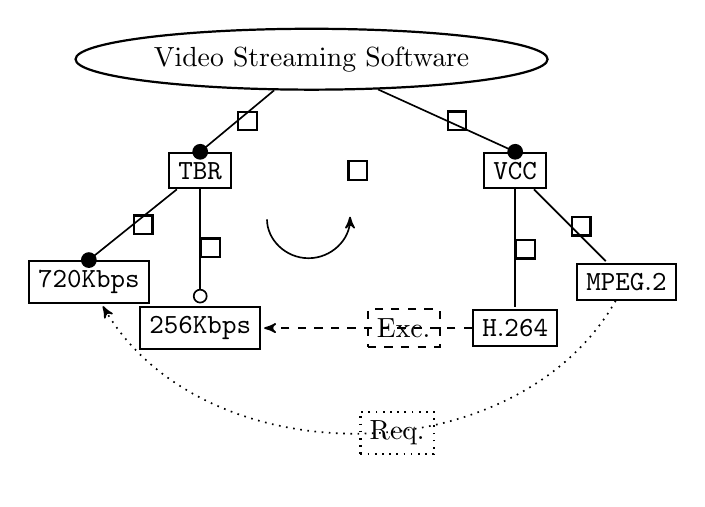
\begin{tikzpicture}[>=stealth',shorten >=1pt,auto,node distance=2cm, semithick,edge from parent]
  \node[ellipse,draw] (A)   {Video Streaming Software};
  \node[rectangle,draw]    (B) [below left  of=A]   {\TXBITRATE};
  \node[]    (AUX) [right  of=B]   {};
  \node[rectangle,draw]    (C) [right   of=AUX]   {\VCC};
  \node[rectangle,draw]    (D) [below left   of=B]   {\STZKPS};
  \node[rectangle,draw]    (E) [below of=B]   {\TFSKPS};
  \node[rectangle,draw]    (F) [below of=C]   {\HTSF};
  \node[rectangle,draw]    (G) [below right of=C]   {\MPEGTWO};

  \path (A) edge [] node {} (B.north)

            edge [] node {} (C.north)

        (B) edge [] node {} (D.north)
            edge [-o, fill] node {} (E)

        (C) edge [] node {} (F)

            edge []  node {} (G)

        (F) edge [->,dashed]  node {Exc.} (E)

        (G) edge [->,dotted,bend left=60]  node {Req.} (D)

  ;

\fill (B.north) circle (-0.1);
\fill (C.north) circle (-0.1);
\fill (D.north) circle (-0.1);
%\fill (-1.3,-1.3) circle (0.1);
%\fill (2.4,-1.3) circle (0.1);
%\fill (-3,-3) circle (0.1);

\draw [<-] (3.5,-2)  arc (360:180:15pt);

%\draw [fill=black](0,-0.35) -- (-0,-0.6) -- (0.6,-0.6)-- (0.35,-0.35)--(0,-0.35);

%\draw [<-] (A.south east)  arc (360:180:14pt);



%\draw [<-] (0.5,-0.2)  arc (360:180:14pt);

%\draw [<-] (-1.1,-4.2)  arc (360:180:14pt);

%\draw [<-] (1.5,-4.2)  arc (360:180:14pt);

%\draw [fill=black](-0.25,-4.85) -- (-0.5,-5.1) -- (0.2,-5.1)-- (0.1,-4.85)--(-0.25,-4.85);

%\draw [fill=black](2.4,-4.85) -- (2.5,-5.1) -- (3.20,-5.1)-- (2.75,-4.85)--(2.35,-4.85);

\end{tikzpicture}
}


\newcommand{\semden}[1]{\ensuremath{[\![#1]\!]}}
\newcommand{\Semden}[1]{\ensuremath{\left[\!\!\left[#1\right]\!\!\right]}}
\newcommand{\semdenp}[1]{\ensuremath{[\![#1]\!]^\calP}}
\newcommand{\Semdenp}[1]{\ensuremath{\left[\!\!\left[#1\right]\!\!\right]^\calP}}
\newcommand{\accum}{\mathtt{accum}}
\newcommand{\menos}{\mathbin{\backslash}}
\newcommand{\op}{\ensuremath{\mathtt{op}}}
\newcommand{\igecu}{\mathbin{=_{E}}}
\newcommand{\vocabulary}[1]{\ensuremath{\mathsf{voc}(#1)}}
\def\spaceFigure{0.3em}
\def\linefigure{\vspace*{\spaceFigure}\hrule\vspace*{\spaceFigure}}



\def\MPEGTWO{\feature{MPEG.2}}
\def\STZKPS{\feature{720Kbps}}
\def\HTSF{\feature{H.264}}
\def\TFSKPS{\feature{256Kbps}}
\def\TXBITRATE{\feature{TBR}}
\def\SHELL{\feature{Shell}}
\def\VCC{\feature{VCC}}
\newcommand\VSS{\feature{VSS}}

\def\oMPEGTWO{\ofeature{MPEG.2}}
\def\oSTZKPS{\ofeature{720Kbps}}
\def\oHTSF{\ofeature{H.264}}
\def\oTFSKPS{\ofeature{256Kbps}}
\def\oTXBITRATE{\ofeature{TBR}}
\def\oSHELL{\ofeature{Shell}}
\def\oVCC{\ofeature{VCC}}

\def\reduction#1{\ensuremath{\mathrm{equation}~#1}}
\newcommand{\EX}[1]{\textbf{#1}}

    \lstnewenvironment{XML}[1][]{
    \lstset{basicstyle=\fontsize{5}{6}\selectfont\ttfamily,
    linewidth=0.90\linewidth,
    %numbers=left,
    stepnumber=1,
    numbersep=10pt,
    %frame=single,
   % framerule=1.0pt,
    backgroundcolor=\color{white},
    language=HTML,
    identifierstyle=\color[rgb]{1,0,0},
    emph={schema, element, complexType, choice, simpleType, sequence, restriction, pattern}, emphstyle=\color{red},
    keywordstyle=\color[rgb]{0,0,1},
    commentstyle=\color[rgb]{0.133,0.545,0.133},
    stringstyle=\color[rgb]{0.627,0.126,0.941},
    morekeywords={xml, ref, xs, version, targetNamespace, minOccurs, maxOccurs}
    }\lstset{#1}}{}
    
    \lstdefinestyle{Bash}
{language=bash,
keywordstyle=\color{blue},
basicstyle=\ttfamily,
morekeywords={peter@kbpet},
alsoletter={:~$},
morekeywords=[2]{peter@kbpet:},
keywordstyle=[2]{\color{red}},
literate={\$}{{\textcolor{red}{\$}}}1 
         {:}{{\textcolor{red}{:}}}1
         {~}{{\textcolor{red}{\textasciitilde}}}1,
}

%%% Local Variables: 
%%% mode: latex
%%% TeX-master: "main"
%%% End: 


%%%
%From macros insof...

\newcommand{\requires}{%
  \def\SeparacionInternaFlecha{-0.3em}
  \def\SeparacionExternaFlecha{-0.5em}
  \def\SeparacionFlechaArriba{-3pt}
  \ensuremath\mathbin{\MacrosTranGeneralProp{\hbox to 2em{\hss}}{\succ}{\cdot\cdot}{}{}}}


%-----------------
% feature

\newcommand{\vars}{\mathsf{vars}}
\newcommand{\maxin}{\mathsf{maxin}}
\newcommand{\logand}{\wedge}
\newcommand{\logimplies}{\mathbin{\rightarrow}}
\newcommand{\logor}{\vee}
\newcommand{\logtrue}{\top}
\newcommand{\logfalse}{\bot}
\newcommand{\logneg}{\neg}

\newcommand{\formula}{\phi}
\newcommand{\contin}{\varpropto}

\newcommand{\clausure}{\mathtt{clausure}}



\def\reduction#1{\ensuremath{\mathrm{equation}~#1}}
\newcommand{\inter}{\ensuremath{\mathsf{int}}}

\newcommand{\calFbot}{\calF_{\bot}}


\newcommand{\fA}{{\feature A}}
\newcommand{\fB}{{\feature B}}
\newcommand{\fC}{{\feature C}}
\newcommand{\fD}{{\feature D}}
\newcommand{\fE}{{\feature E}}
\newcommand{\fF}{{\feature F}}
\newcommand{\fG}{{\feature G}}
\newcommand{\fH}{{\feature H}}
\newcommand{\fI}{{\feature I}}
\newcommand{\fL}{{\feature L}}
\newcommand{\fM}{{\feature M}}
\newcommand{\fN}{{\feature N}}
\newcommand{\fO}{{\feature O}}
\newcommand{\fP}{{\feature P}}
\newcommand{\fQ}{{\feature Q}}
\newcommand{\fR}{{\feature R}}
\newcommand{\fS}{{\feature S}}
\newcommand{\fT}{{\feature T}}
\newcommand{\fU}{{\feature U}}
\newcommand{\fV}{{\feature V}}


\newcommand{\ofA}{\ofeature{A}}
\newcommand{\ofB}{\ofeature{B}}
\newcommand{\ofC}{\ofeature{C}}
\newcommand{\ofD}{\ofeature{D}}
\newcommand{\ofE}{\ofeature{E}}
\newcommand{\ofF}{\ofeature{F}}
\newcommand{\ofG}{\ofeature{G}}
\newcommand{\ofH}{\ofeature{H}}
\newcommand{\ofI}{\ofeature{I}}

% \newcommand{\lbag}{\langle}
% \newcommand{\rbag}{\rangle}

\newcommand{\natbot}{\nat_\bot}

\newcommand{\icost}{\ensuremath{\mathtt{c}}}
\newcommand{\cost}[1]{\icost(#1)}
\newcommand{\costt}[1]{\ensuremath{\mathtt{t\icost}(#1)}}
\newcommand{\costfoda}{\icost_{\fodaPA}}
\newcommand{\minc}[1]{\ensuremath{\mathtt{minc}(#1)}}

\def\novtran#1{\ensuremath\mathbin{\MacrosNoVTran{#1}}}
\def\tranold#1{\ensuremath\mathbin{\MacrosTran{#1}_{\!\!\!\!o\;}}}
\def\trannew#1{\ensuremath\mathbin{\MacrosTran{#1}_{\!\!\!\!n\;}}}

\newcommand{\productsnew}[1]{\ensuremath{\mathtt{prod}_n\left(#1\right)}}
\newcommand{\productsold}[1]{\ensuremath{\mathtt{prod}_o\left(#1\right)}}
\newcommand{\tracesnew}[1]{\ensuremath{\mathtt{tr}_n(#1)}}
\newcommand{\tracesold}[1]{\ensuremath{\mathtt{tr}_o(#1)}}

\newcommand{\runlist}{\ensuremath{\mathit{run\mbox{-}list}}}



    \newcommand*\circled[1]{\tikz[baseline=(char.base)]{
            \node[shape=circle,draw,inner sep=2pt] (char) {#1};}}
            
\tikzstyle{every node}=[draw=black,thick,anchor=west]
\tikzstyle{selected}=[draw=red,fill=red!30]
\tikzstyle{optional}=[dashed,fill=gray!50]
\lstset{language=Ruby,frame=trBL,basicstyle=\ttfamily\fontsize{6}{8}\selectfont}


\title{Probalisitic Software product lines\tnoteref{t1}}
% \tnotetext[t1]{Research partially supported by the Spanish MEC project
%   ESTuDIo (TIN2012-36812-C02-01), 
%   the Comunidad de Madrid project SICOMORo-CM (S2013/ICE-3006) and the
%   UCM-Santander program to fund research groups (group 910606).
% }


% \author[ucm]{Carlos Camacho\corref{cor1}}
% \ead{carlos.camacho@ucm.es}

% \author[ucm]{Luis Llana}
% \ead{llana@ucm.es}

% \author[ucm]{Alberto Núñez}
% \ead{alberto.nunez@pdi.ucm.es}% \author[ucm]{Manuel Núñez}
% \ead{alberto.nunez@pdi.ucm.es}

% \cortext[cor1]{Principal corresponding author}
% \address[ucm]{Universidad Complutense de Madrid, Madrid 28040, Spain}



\begin{document}
%\linenumbers

\begin{abstract}
We introduce a probabilistic extension of our previous
work \fodaPA: a formal framework to specify and analyze software product lines.
We use probabilistic information to identify those features that are more frequently used. This is done by computing the probability of having a feature in a specific software product line.
We redefine the syntax of \fodaPA\ to include probabilistic operators and define new operational and denotational semantics. We prove that the expected equivalence between these two semantic frameworks holds.
Our probabilistic framework is supported by a tool. We briefly comment on the characteristics of the tool and discuss the advantages of using probabilities to quantify the likelihood of having features in potential software product lines.
\end{abstract}
\textbf{Keywords;} Software Product Lines; Probabilistic Models; Formal Methods; Feature Models


%%% Local Variables:
%%% mode: latex
%%% TeX-master: "main"
%%% End:


% $Id: introduction.tex,v 1.8 2013/12/03 09:17:27 ccamacho Exp $
\section{Introduction}
\label{ref:introduction}

%The main purpose of Software Product Lines (in short, \SPLs) is to produce products
%while increasing productivity and shortening the time-to-market period. \SPLs\ depend
%on which software products are being produced and which of them are better for
%a specific criterion. When products are represented in a product line organization,
%several modeling approaches can be used to increase both quality and productivity.
%In most cases this is represented in the form of features, relationships and
%constraints. For instance, some of these approaches are FODA~\cite{kchnp90},
%RSEB~\cite{mj98} and PLUSS~\cite{k05,ebb06}.

During the last years, software product lines (in short, \SPLs) have become a widely adopted mechanism for efficient software development. The Carnegie Mellon Software Engineering Institute defines an \SPL\ as ``a set of software-intensive systems that share a common, managed set of features satisfying the specific needs of a particular market segment or mission and that are developed from a common set of core assets in a prescribed way.'' Basically, the main goal of \SPLs\ is to increase the productivity for creating software products, which is achieved by selecting those software systems that are better for a specific criterion (e.g. a software system is less expensive than others, it requires less time to be processed, etc). Currently, different approaches for representing the product line organization can be found in the literature, such as FODA~\cite{kchnp90},
RSEB~\cite{mj98} and PLUSS~\cite{k05,ebb06}.

Graphical approaches are commonly used to model \SPLs. Feature Oriented Domain Analysis~\cite{kchnp90} (in short, \FODA) is a well-known graphical approach for representing commonality and variability of systems. Figure~\ref{fig:foda:relations} shows all \FODA\ relationships and constraints.
% and Figure~\ref{section:introduction:figure:examples}
% shows some examples of how
% \FODA\ diagrams are built.
Although this kind of solutions is useful to easily model \SPLs, a formal approach is needed for automatizing the analysis process and detecting errors in the early stages of the production process. It is therefore required that graphical representations are translated into mathematical entities~\cite{nak10}. In this case, the original graphical representation of \FODA\ must be provided with a formal semantics~\cite{bhst04}.
%
This  issue is solved by using \fodaPA~\cite{acl13}, a formal framework to represent \FODA\ diagrams using process algebras. \fodaPA\ can be applied not only to \FODA, but also to represent other feature-related problems and variability models. Additionally, some of the existing formal approaches use algebras and semantics~\cite{szw05,kkm06,prb11,acl13}, while others use either propositional or first order logic~\cite{man02,ka07,abgf10,atfg10,nnz14}.

\begin{figure}[t]

\linefigure

\centering


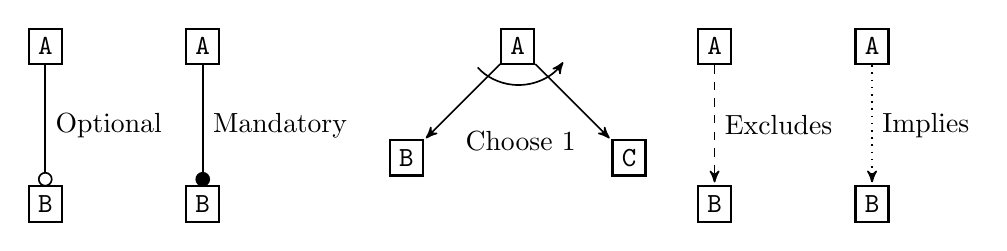
\begin{tikzpicture}[>=stealth',shorten >=1pt,auto,node distance=2cm, semithick]

  \node[rectangle,draw] (A)   {\feature{A}};
  \node[rectangle,draw] (B) [below of=A]   {\feature{B}};

  \node[rectangle,draw] (C) [right of=A]   {\feature{A}};
  \node[rectangle,draw] (D) [below of=C]   {\feature{B}};

%  \node[] (E) [right of=C]   {};
  \node[rectangle,draw,node distance=4cm] (G) [right of=C]   {\feature{A}};
  \node[rectangle,draw] (F) [below left of=G]   {\feature{B}};
%  \node[] (H) [below of=G]   {};
  \node[rectangle,draw] (I) [below right  of=G]   {\feature{C}};



  \path (A) edge [-o,shorten >=-0.05em] node[draw=none] {Optional} (B.north)
        (C) edge [-*,shorten >=-0.05em] node[draw=none] {Mandatory} (D.north)

        (G) edge [->]  node[draw=none, shift={(80:-0.5)}]{Choose 1} (F)
            edge [->]  node[draw=none] {} (I)  ;


\draw [<-] (6.8,-0.2) arc (-36:-140:20pt);

  \node[rectangle,draw,node distance=2.5cm] (J) [right of=G]   {\feature{A}};
  \node[rectangle,draw] (K) [below of=J]   {\feature{B}};

  \node[rectangle,draw] (L) [right of=J]   {\feature{A}};
  \node[rectangle,draw] (M) [below of=L]   {\feature{B}};


  \path
        (J) edge [->,dashed] node[draw=none] {Excludes} (K)
        (L) edge [->,dotted] node[draw=none] {Implies} (M)  ;

\end{tikzpicture}

\linefigure

\caption{\FODA\ Diagram representation.\label{fig:foda:relations}}

\end{figure}


% \begin{figure}[t]
% \linefigure
% \centering
% \begin{minipage}{0.2\hsize}
%         \centering
%         \EX{a}


%         \centering
%         \begin{tikzpicture}[>=stealth',shorten >=1pt,auto,node distance=1.5cm, semithick]

%           \node[rectangle,draw] (A)   {\feature{A}};
%           \node[rectangle,draw,node distance=1.1cm] (B) [below of=A]   {\feature{B}};

%           \path (A) edge [-o] node[draw=none] {} (B.north)
%           ;
%         \end{tikzpicture}

% \end{minipage}
% %
% \begin{minipage}{0.1\hsize}

%         \centering

%         \EX{b}

%         \begin{tikzpicture}[>=stealth',shorten >=1pt,auto,node distance=1.5cm, semithick]


%           \node[rectangle,draw] (C) [right of=A]   {\feature{A}};
%           \node[rectangle,draw,node distance=1.1cm] (D) [below of=C]   {\feature{B}};
%           \path (C) edge [] node[draw=none] {} (D)
%           ;
%         \fill (D.north) circle (0.1);
%         \end{tikzpicture}

% \end{minipage}
% %
% \begin{minipage}{0.33\hsize}
% \centering

%         \EX{c}

%         \begin{tikzpicture}[>=stealth',shorten >=1pt,auto,node distance=1.5cm, semithick]


%           \node[rectangle,draw] (G)    {\feature{A}};
%           \node[rectangle,draw] (F) [below left of=G]   {\feature{B}};
%           \node[rectangle,draw] (I) [below right  of=G]   {\feature{C}};

%           \path
%                 (G) edge [->]  node[draw=none] {} (F)
%                     edge [->]  node[draw=none] {} (I)

%           ;

%         \draw [<-] (0.7,-0.1) arc (360:180:14pt);

%         \end{tikzpicture}
% \end{minipage}
% \begin{minipage}{0.33\hsize}
% \centering

%         \EX{d}


%         \begin{tikzpicture}[>=stealth',shorten >=1pt,auto,node distance=1.5cm, semithick]
%           \node[rectangle,draw] (G)   {\feature{A}};

%           \node[rectangle,draw] (F) [below left of=G]   {\feature{B}};
%           \node[rectangle,draw] (I) [below right  of=G]   {\feature{C}};
%           \path
%                 (G) edge []  node[draw=none] {} (F.north)
%                     edge []  node[draw=none] {} (I.north)
%           ;
%         \fill (F.north) circle (0.1);
%         \fill (I.north) circle (0.1);
%         \end{tikzpicture}
% \end{minipage}


% \linefigure



% \begin{minipage}{0.33\hsize}
% \centering
%         \EX{e}
% \vspace*{0.3em}

%         \begin{tikzpicture}[>=stealth',shorten >=1pt,auto,node distance=1.5cm, semithick]
%           \node[rectangle,draw] (G)    {\feature{A}};
%           \node[rectangle,draw] (F) [below left of=G]   {\feature{B}};
%           \node[rectangle,draw] (I) [below right  of=G]   {\feature{C}};
%           \path
%                 (G) edge [-o]  node[draw=none] {} (F.north)
%                     edge []  node[draw=none] {} (I.north) ;
%         \fill (I.north) circle (0.1);
%         \end{tikzpicture}
% \end{minipage}
% \begin{minipage}{0.3\hsize}
%         \centering
%  \EX{f}

%         \begin{tikzpicture}[>=stealth',shorten >=1pt,auto,node distance=1.5cm, semithick]


%           \node[rectangle,draw] (A)    {\feature{A}};
%           \node[rectangle,draw] (B) [below left   of=A]   {\feature{B}};
%           \node[rectangle,draw] (C) [below right  of=A]   {\feature{C}};

%           \path
%                 (A) edge [-o]  node[draw=none] {} (B.north)
%                         edge [-o]  node[draw=none] {} (C.north)

%     (B) edge [->,dashed] node[draw=none] {} (C);
%         \end{tikzpicture}
% \end{minipage}
% \begin{minipage}{0.3\hsize}
%         \centering
%  \EX{g}

%         \begin{tikzpicture}[>=stealth',shorten >=1pt,auto,node distance=1.5cm, semithick]


%           \node[rectangle,draw] (A)    {\feature{A}};
%           \node[rectangle,draw] (B) [below left   of=A]   {\feature{B}};
%           \node[rectangle,draw] (C) [below right  of=A]   {\feature{C}};

%           \path
%                 (A) edge [-o]  node[draw=none] {} (B.north)
%                         edge [-o]  node[draw=none] {} (C.north)

%         (B) edge [->,dotted] node[draw=none] {} (C)
% ;
%         \end{tikzpicture}
% \end{minipage}
% \linefigure

% \caption{Examples of \FODA\ Diagrams.\label{section:introduction:figure:examples}}
% \end{figure}

%Feature Oriented Domain Analysis~\cite{kchnp90} (in short, \FODA) is a graphical
%representation of commonality and variability of systems. Figure~\ref{fig:foda:relations}
%shows all \FODA\ relationships and constraints.
%% and Figure~\ref{section:introduction:figure:examples}
%% shows some examples of how
%% \FODA\ diagrams are built.
%In order to perform automatic analysis,  graphical representations
%must be transformed into mathematical entities~\cite{nak10}.
%Thus, it is necessary to provide the original
%\FODA\ graphical representation with formal semantics base, where automated analysis can be
%performed~\cite{bhst04}. This  issue is solved by using \fodaPA~\cite{acl13}, a formal
%framework to represent \FODA\ diagrams using process algebras. \fodaPA\
%can only be applied not only to
%\FODA, but also to represent other feature-related
%problems and variability models.

%Costs within our formal framework refer to the required effort to add a feature to a product
%under construction. This cost refers to many factors depending on the context of the
%product line organization. For example, the cost of adding a feature to a product can be
%equal to the number of lines of code of a software component~\cite{n07,babc09}, or the
%effort, in terms of human hours, to develop that module. This effort is usually measured by using
%functional metrics~\cite{j04,cg08,hko13}. The cost of adding third-party modules, both
%commercial and open source, to our \SPL\ could be the time associated with integrating it into
%the product line organization.

%The order in which features are computed is important in many software projects and
%has an  important relevance to the final cost of the project. This order can be easily incorporated
%into the operational semantics of~\fodaPA. In this paper we represent costs with
%natural numbers. This is not a drawback of our formalism because we can assume a
%minimum cost unit, and therefore, any cost can be represented as a multiple of this unit.

It is worth to mention that the order in which features are processed to create a specific product is directly reflected in its final cost. In a previous work we introduced costs in our formal framework for representing the required effort to include a feature to the product under construction~\cite{cln16}. This cost may represent different aspects of a feature, such us lines of code of a given software component or effort, in human hours, to include a software component into a project, just to name a few, that usually depends on the target of the product line organization. Thus, efficiently processing features for building high quality products becomes a time-consuming and challenging task. Unfortunately, there are some situations where the representation of the \SPL\ generates a combinatorial explosion, making unpractical to analyze all possible combinations.
%
In order to alleviate this issue, we propose a probabilistic extension of our previous work \fodaPA. We use probabilistic information to identify those features that are more frequently used by computing the probability of having a feature in a specific \SPL. Hence, the computation is focused on those features with a high probability to be present in the final product, reducing the total computation required for generating valid products.




The study of probabilistic extensions of formal methods can be dated back to the end of the 1980s. This is already a well established area, with many long contributions extending classical formalisms (Process Algebras, I/O Automata, Finite State Machines, Input Output Transition Systems, among others) to include probabilistic information~\cite{ls91,rgs95,cdsy99,nun03,lnr06,csv07,dghm08,hm09,hn10,dghm14,agl16}.
%
%
\mncomment{He comentado la figura y la explicacion porque este modelo no se parece en nada al que genera la semantica operacional: en nuestro caso, las transiciones tienen accion y probabilidad.}
%Figures like the displayed trees describe how probabilities are assigned in the system behavior (see Figure~\ref{fig:displayedTrees}). These models allow to assign a real value between 0 and 1 to each transition in order to execute an event. It is important to notice that the probability of execute a transition \textit{t} is not necessarily equal to the other probabilities from the same level.
%\begin{figure}[h]
%	\hspace{50px}
%	\begin{minipage}{0.4\hsize}       		
%		
%		\begin{minipage}{0.2\hsize}
%			\scalebox{0.6}{
%				\begin{tikzpicture}[>=stealth',shorten >=1pt,auto,node distance=2cm, semithick]
%				
%				\node[circle,draw] (A)   {};
%				\node[circle,draw] (B) [below left of=A]   {};
%				\node[regular polygon,regular polygon sides=3,draw,scale=0.8] (F) [below of=B]   {T};
%				\node[circle,draw] (C) [below right of=A]   {};
%				\node[circle,draw] (D) [below left of=C]   {};
%				\node[circle,draw] (E) [below right of=C]   {};
%				\node[regular polygon,regular polygon sides=3,draw,scale=0.8] (G) [below  of=D]   {T};
%				\node[regular polygon,regular polygon sides=3,draw,scale=0.8] (H) [below  of=E]   {T};			 
%				
%				\path (A) edge [] node [pos=0.5, above left, draw=white, opacity=0, text opacity=1]{1/3} (B);
%				\path (B) edge [] node [pos=0.5, left, draw=white, opacity=0, text opacity=1]{a} (F);
%				\path (A) edge [] node [pos=0.5, above right, draw=white, opacity=0, text opacity=1]{1/2} (C);
%				\path (C) edge [] node [pos=0.5, above left, draw=white, opacity=0, text opacity=1]{1/2} (D);
%				\path (C) edge [] node [pos=0.5, above right, draw=white, opacity=0, text opacity=1]{1/2} (E);
%				\path (D) edge [] node [pos=0.5, right, draw=white, opacity=0, text opacity=1]{b} (G);
%				\path (E) edge [] node [pos=0.5, left, draw=white, opacity=0, text opacity=1]{c} (H);
%				\end{tikzpicture}
%			}
%		\end{minipage}
%	\end{minipage}
%	\begin{minipage}{0.4\hsize}
%		
%		\begin{minipage}{0.2\hsize}
%			\scalebox{0.6}{
%				\begin{tikzpicture}[>=stealth',shorten >=1pt,auto,node distance=4cm, semithick]
%				\node[circle,draw] (A)   {};
%				\node[regular polygon,regular polygon sides=3,draw,scale=0.8] (B) [below left of=A]   {T};
%				\node[regular polygon,regular polygon sides=3,draw,scale=0.8] (C) [below  of=A]   {T};			 
%				\node[regular polygon,regular polygon sides=3,draw,scale=0.8] (D) [below right of=A]   {T};			 
%				
%				\path (A) edge [] node [pos=0.5, above left, draw=white, opacity=0, text opacity=1]{1/3} (B);
%				\path (A) edge [] node [pos=0.5, left, draw=white, opacity=0, text opacity=1]{1/3} (C);
%				\path (A) edge [] node [pos=0.5, above right, draw=white, opacity=0, text opacity=1]{1/3} (D);
%				
%				\end{tikzpicture}}
%		\end{minipage}
%		
%	\end{minipage}
%	
%	\caption{Displayed trees representing probabilities.}
%	\label{fig:displayedTrees}
%	
%\end{figure}
%
%\acomen{He puesto título y referencia a esta figura (Fig. 2). Please, check!}
%
\acomen{Carlos, he cambiado el siguiente texto con referencias a papers de probabilidades. Please, check para ver que no digo nada cantoso)}
%
Several works in the literature show that statistic analysis over \SPLs\ allow to determine relevant characteristics, like the certainty of finding valid products among complex models~\cite{tllv15,tlll15,chssgl13,dpcslsh17}.
%
Some of these works describe models to run statistical analysis over \SPLs, where pre-defined syntax elements are computed by applying a specific set of operational rules~\cite{tllv15,tlll15}. These models demonstrate their ability to be integrated into standard tools like QFLan, Microsoft's SMT Z3 and MultiVeStA.
%
%Some of these works describe models to run statistical analysis to represent \SPLs\ by defining an specific set of operational rules to compute their defined syntax elements~\cite{tllv15,tlll15}. These models demonstrate their ability by being integrated to standard tools like QFLan, Microsoft's SMT Z3 and MultiVeStA.
%
Cordy et al. focus on testing properties of \SPLs, like reliability, which defines three verification techniques, a probabilistic model checker on each product, on a model range, and testing the behavior relations with other models~\cite{chssgl13}. Other works focus on describing use cases for analyzing the probability of finding features inside valid products~\cite{dpcslsh17}. %An interesting feature is that any of the referenced research articles describe their approaches using multisets.

The rest of the paper is structured as follows. Section \ref{sec:stat:sintaxMain} presents our language. Section \ref{sec:equivalenceMain} describes the equivalence between the operational and denotational semantics. In section \ref{sec:stat:hidMain} we describe how the sets of features are hidden. Section~\ref{sec:stat:impl} shows our implementation of the denotational semantics for the probabilistic extension. Finally, section~\ref{section:jstat:concs} presents our conclusions and some future work.

\acomen{He cambiado el nombre de secciones (label) repetidas. Please, check!.}

%%% Local Variables:
%%% mode: latex
%%% TeX-master: "main"
%%%   ispell-local-dictionary: "american"
%%% End:



% LocalWords:  formalisms

\section{$\fodaPAp$: syntax and semantics}
\label{sec:stat:sintaxMain}
In this section we introduce our language. In addition to present its syntax, we define an operational semantics and a denotational semantics. In the next section we will show the equivalence between these two semantic frameworks.


\subsection{Syntax and operational semantics}
\label{sec:stat:sintax}
Following our previous work~\cite{acl13,clc16}, we will consider a
set of features. We denote this set by $\calF$ and consider that $\feature{A}, \feature{B},
\feature{C}$ range over $\calF$. We have a special feature
$\checkmark\not\in\calF$ to mark the end  of a product. We consider a syntax similar to
\fodaPA, where probabilities are introduced both in the choice operator $P \choice_{p} Q $ and in
the optional feature operator $\ofeature{A};_{p} P$. We do not allow
\emph{degenerated} probabilities, that is, for all probability $p$ we have $0< p<1$.

The operators syntax is defined as in~\cite{acl13,clc16}.
In order to define the syntax, 
we need to fix the set of \emph{features}. 
From now on $\calF$ denotes a finite set  of features
and  \feature{A}, \feature{B}, \feature{C}\dots\ denote isolated features.

In the syntax of the language there are two sets of operators. 
On the one hand there are \emph{main operators}, such as $\cdot\choice\cdot$, $\cdot\paral\cdot$, $\feature{A};\cdot$, $\ofeature{A};\cdot$, 
$\require{A}{B}{\cdot}$, $\exclude{A}{B}{\cdot}$,
that directly correspond to relationships in \FODA\ diagrams.
On the other hand, we have \emph{auxiliary operators}, such as $\nil$, $\checkmark$, $\forbid{A}{\cdot}$, $\mandatory{A}{\cdot}$,
which we need to define the semantics of the language.


\bdfn
\label{sec:stat:sintax:dfn}
A \emph{probabilitistc SPL} is a term generated by the following
BNF expression:
$$
\begin{array}{ll}
P::=& \checkmark \barra \nil \barra \feature{A};P \barra
\ofeature{A};_{p} P \barra P \choice_{p} P \barra P \paral P \barra
\\
& \exclude{A}{B}{P}\barra  \require{A}{B}{P}\barra  \forbid{A}{P}\barra  \mandatory{A}{P}\\
\end{array}
$$
\noindent
where $\feature{A},\feature{B} \in \calF$ and $p\in(0,1)$. The set of terms of the
algebra will be denoted by  $\fodaPAp$.
\edfn



In order to avoid writing too many parentheses in the terms, we 
assume left-associativity in binary operators and  the
following precedence in the operators (from higher to lower priority):
$\feature{A};P$, $\ofeature{A};_{p} P$, $ P \choice_{p} Q$, $P\paral Q$,
$\exclude{A}{B}{P}$, $\require{A}{B}{P}$, 
$\require{A}{B}{P}$,  $\forbid{A}{P}$, and $\mandatory{A}{P}$.
In~\cite{acl13,clc16} we demonstrated that
the binary
operators are commutative and associative.
As a result, the
\emph{choose-one} operator ($\cdot\choice_{p}\cdot$) and the
\emph{conjunction} operator ($\cdot\paral\cdot$) are $n$-ary operators
instead of just binary operators. 


The Extended BNF in Definition~\ref{sec:stat:sintax:dfn} says
that a term of \fodaPA\ is
a sequence of operators and features.

There are two terminal symbols in
the language, $\nil$ and $\checkmark$,
we need them to define the semantics of the language.
%, see 
%The first semantics where we will use them will be an \emph{operational} semantics.
Let us note that the products of a term in \fodaPA\ will be computed following some rules.
The computation will finish when no further steps are allowed. 
This fact is represented by the $\nil$ symbol. 
We will introduce rules to compute a product, with this computation
finishing when no further steps are required, a situation represented by~\nil.
During the computation of an \fodaPAp\ term,  we have 
to represent the situation in which a \emph{valid product} 
of the term has been computed. 
This fact is represented by the $\checkmark$ symbol.

The operators $\feature{A};P$ and $\ofeature{A}_{p};P$ add the feature $\feature{A}$ to any product that can be obtained
from $P$. The operator $\feature{A};P$ indicates that $\feature{A}$ is mandatory while $\ofeature{A}_{p};P$ indicates
that $\feature{A}$ is optional and computed with probability $p$.
There are two binary operators: $P \choice_{p} Q$ and $P\paral Q$. The
first one represents the \emph{choose-one} operator while the second one represents the  \emph{conjunction} operator.

The constraints are easily represented in \fodaPAp.
The operator $\require{A}{B}{P}$ represents the \emph{require}
constraint in \FODA.
The operator $\exclude{A}{B}{P}$ represents the \emph{exclusion}
constraint in \FODA.  

The operator $\mandatory{A}{P}$ is necessary to define the behavior
of the $\require{A}{B}{P}$ operator:
when we compute the products of the term $\require{A}{B}{P}$, we have 
to take into account whether  product  \feature{A} has been produced or not.
In the case it has been produced, we have to annotate 
that we need to produce \feature{B} in the future.
The operator $\mandatory{B}{P}$  is used for this purpose.
The same happens with  the operator $\forbid{B}{P}$.
% is necessary to define the semantics of the $\exclude{A}{B}{P}$.
When we  compute the products of $\exclude{A}{B}{P}$,   
if the feature \feature{A} is computed
at some point, we  annotate
that \feature{B} must not be included. The operator $\forbid{B}{P}$ indicates
that product \feature{B} is forbidden.






























%\todo{Hay que explicar los operadores probabilísticos $P \choice_{p}
%       Q$ y $\ofeature{A};_{p} P$ y la razón por la que el resto no
%       necesita probabilidades.}

%%% Local Variables:
%%% mode: latex
%%% TeX-master: "main"
%%% End:

%\subsection{Operational Semantics}
%\label{sec:stat:oper}


\begin{figure*}[h]
        \linefigure

        \centering\scalebox{0.95}{%
        $
        \begin{array}{*{3}{l@{}c@{\hspace{4em}}}}
        \nombreRegla{tick} & \checkmark\tranp{\checkmark}{1}\nil &
        \nombreRegla{feat} & \feature{A};P\tranp{\feature{A}}{1}P \\
        \nombreRegla{ofeat1} & \ofeature{A};_{p}P\tranp{\feature{A}}{p}P &
        \nombreRegla{ofeat2} & \ofeature{A};_{p}P\tranp{\checkmark}{(1-p)}\nil\\
        \nombreRegla{cho1} & \displaystyle \frac{P\tranp{\feature{A}}{p} P_1}{P\choice_{q} Q\tranp{\feature{A}}{p\cdot q} P_1}&
        \nombreRegla{cho2} & \displaystyle\frac{Q\tranp{\feature{A}}{q} Q_1}{P\choice_{p} Q\tranp{\feature{A}}{(1-p)\cdot q}Q_1}\\
        \nombreRegla{con1} & \displaystyle\frac{P\tranp{\feature{A}}{p} P_1}{P\paral Q\tranp{\feature{A}}{\frac{p}{2}}P_1\paral Q} &
        \nombreRegla{con2} & \displaystyle\frac{Q\tranp{\feature{A}}{q} Q_1}{P\paral Q\tranp{\feature{A}}{\frac{q}{2}}P\paral Q_1}\\
        \nombreRegla{con3} & \displaystyle\frac{P\tranp{\checkmark}{q}\nil, Q\tranp{\checkmark}{p}\nil}{P\paral Q\tranp{\checkmark}{p\cdot q}\nil} &\\
        \nombreRegla{con4} & \displaystyle\frac{P\tranp{\feature{A}}{p} P_1, Q\tranp{\checkmark}{q}\nil}{P\paral Q\tranp{\feature{A}}{\frac{p\cdot q}{2}} P_1} &
        \nombreRegla{con5} & \displaystyle\frac{P\tranp{\checkmark}{p}\nil,Q\tranp{\feature{A}}{q} Q_1}{P\paral Q\tranp{\feature{A}}{\frac{p\cdot q}{2}} Q_1} \\
        %
        %
        \nombreRegla{req1} & \displaystyle
        \frac{P \tranp{\feature{C}}{p} P_1,\ \feature{C}\neq\feature{A}}{\require{A}{B}{P}
                \tranp{\feature{C}}{p} \require{A}{B}{P_1}} &
        \nombreRegla{req2} &  \displaystyle
        \frac{P \tranp{\feature{A}}{p} P_1}{\require{A}{B}{P}\tranp{\feature{A}}{p} \mandatory{B}{P_1}} & \\
        % \nombreRegla{req3} & \displaystyle
        % \frac{P \tranp{\feature{B}}{p} P_1}{\require{A}{B}{P}
        %   \tranp{\feature{B}}{p} P_1} &
        \nombreRegla{req3} &  \displaystyle
        \frac{P \tranp{\feature{\checkmark}}{p} \nil}{\require{A}{B}{P}
                \tranp{\feature{\checkmark}}{p} \nil}\\
        \nombreRegla{excl1} &    \displaystyle
        \frac{P \tranp{\feature{C}}{p} P_1,\ \feature{C}\neq\feature{A},\  \feature{C}\neq\feature{B}}{
                \exclude{A}{B}{P}\tranp{\feature{C}}{p} \exclude{A}{B}{P_1}} &
        \nombreRegla{excl2} & \displaystyle
        \frac{P \tranp{\feature{A}}{p} P_1}{\exclude{A}{B}{P}
                \tranp{\feature{A}}{p}\forbid{B}{P_1}} \\
        \nombreRegla{excl3} & \displaystyle
        \frac{P \tranp{\feature{B}}{p} P_1}{\exclude{A}{B}{P}\tranp{\feature{B}}{p}\forbid{A}{P_1}}
        &
        \nombreRegla{excl4} & \displaystyle
        \frac{P \tranp{\checkmark}{p} \nil}{\exclude{A}{B}{P}\tranp{\checkmark}{p}\nil}\\

        \nombreRegla{forb1} & \displaystyle
        \frac{P \tranp{\feature{B}}{p} P_1,\ \feature{B}\neq\feature{A}}{\forbid{A}{P}
                \tranp{\feature{B}}{p} \forbid{A}{P_1}} &
        \nombreRegla{forb2} & \displaystyle
        \frac{P \tranp{\checkmark}{p} \nil}{\forbid{A}{P}
                \tranp{\checkmark}{p} \nil}  \\
        %      \nombreRegla{forb3} & \displaystyle
        %     \frac{P\tran{\feature{A}}P_2 \tran{\feature{F}} P_1}{\forbid{A}{P}
        %       \tran{\feature{B}} \forbid{A}{P_1}},\ \feature{B}\neq\feature{A} &
        %      \nombreRegla{forb4} & \displaystyle
        %     \frac{P\tran{\feature{A}}P_2 \tran{\feature{\checkmark}} P_1}{\forbid{A}{P}
        %       \tran{\checkmark} \nil}\\
        %
        %
        %
        \nombreRegla{mand1} &  \displaystyle\frac{P\tranp{\checkmark}{p} \nil}{\mandatory{A}{P}
                \tranp{\feature{A}}{p} \checkmark}  &
        \nombreRegla{mand2} &  \displaystyle\frac{P\tranp{\feature{A}}p P_1}{\mandatory{A}{P}\tranp{\feature{A}}p P_1} \\
        \nombreRegla{mand3} &  \displaystyle\frac{P\tranp{\feature{B}}p
                P_1,\ \feature{A}\neq\feature{B}}{\mandatory{A}{P}\tranp{\feature{B}}p \mandatory{A}{P_1}}
        \\
        \multicolumn{4}{c}{\feature{A},\feature{B},\feature{C}\in\calF,\ a\in\calF\cup\{\checkmark\}}

        \end{array}
        $}

        \noindent

        \linefigure

        \caption{\fodaPAp\ operational semantics.  \label{fig:sos-rules}}
\end{figure*}

\mncomment{No he leido la semantica operacional con cuidado: confio en Luis :-)}
%
In Figure~\ref{fig:sos-rules} we present the set of rules formally defining  the operational behavior of
\fodaPAp. These rules essentially coincide with the ones corresponding
\fodaPA~\cite{acl13}, but with the addition of probabilities. Next we focus 
on the explanation of the role of probabilities. Rules
$\nombreRegla{tick}$ and $\nombreRegla{feat}$
show the corresponding feature with probability 1.
%
Rules  $\nombreRegla{ofeat1}$ and $\nombreRegla{ofeat2}$ deal with the
probabilistic optional feature. The feature can be chosen with probability
$p$ and can be rejected with probability  $1-p$. Let us note that both probabilities
are not null.
%
Rules $\nombreRegla{cho1}$ and $\nombreRegla{cho2}$ define the
behavior of the probabilistic choice operator. The left branch is
selected with probability $p$ and the right with probability $1-p$.
%
It is important to note rules for the conjunction operator
(Rules $\nombreRegla{con1}$ to $\nombreRegla{con4}$)
distribute the probability equitably between both
branches, that is, $\frac{1}{2}$. We have preferred to use a simple definition of this operator, but it is easy to replace it by a more involved version of a probabilistic parallel operator~\cite{ahk98}.
%
Rule $\nombreRegla{con5}$ requires that both branches agree on the
termination of a product.
%
We use \emph{multisets} of transitions to consider different occurrences of the same transition. So, if a transition can be derived in several ways, each derivation generates a different
instance of this transition. For example, let us consider the
term
$P=\ofeature{A} \choice_{\frac12} \ofeature{A}$, where trailing occurrences of
$\nil$ have been omitted. If we were not careful, we would have
the transition $P\tranp{\feature{A}}{\frac12}\nil$ only once, while we
should have this transition twice. So, if a transition can be derived in
several ways, we consider that each derivation generates a
different instance. In particular, we will later consider multisets of computations as well.
%
We will use the delimiters~$\lbag$ and~$\rbag$ to denote
multisets.\mncomment{donde estan definidos $\lbag$ and~$\rbag$?? Poned una notacion standard, algo del estilo $\{ \!\!\!\:|\;$ y $\;| \!\!\!\:\}$}

The following result, the proof is immediate, show that successful termination leads to $\nil$.
\mncomment{Esto pa que sirve? Es obvio, no?}

\blem\label{lem:check}
Let $P,Q\in\fodaPAp$ and $p\in(0,1]$. We have $P\tranp{\checkmark}{p}{Q}$ if and only if $Q=\nil$.
\elem

Next we present some notions associated with the composition of consecutive transitions. 

\bdfn\label{def:trtrantions} Let $P,Q\in\fodaPAp$. We write  $P\vtranp{s}{p}Q$ if there exist a sequence of consecutive transitions
\begin{displaymath}
    P=P_0\tranp{a_1}{p_1}P_1\tranp{a_2}{p_2}P_2\cdots P_{n-1}\tranp{a_n}{p_n} P_n=Q
\end{displaymath}
where $n\geq 0$, $s=a_1a_2\cdots a_n$ and $p=p_1\cdot p_2\cdot \cdots p_{n}$.

Let $P\in\fodaPAp$. We define the set of probabilistic products of $P$, denoted by $\prodp(P)$, as the set
\begin{displaymath}
\{(pr,p)\ |\ p>0 \wedge p=\sum\lbag q\ |\
  P\vtranp{s\checkmark}{q} Q \y \product{s}=pr \rbag\}
\end{displaymath}
\mncomment{$\product{s}$ no definido! Ya os digo yo que no se puede asumir que el PC son mega-expertos en SPL}
\item We define the total probability of $P$, denoted by $\ham(P)$, as $\rbag p\ |\ \exists pr: (pr,p)\in\prodp(P)$. In addition, we define $\waste(P) = 1-\ham(P)$.
\edfn

The following result shows some properties, concerning probabilities, of the operational semantics. In particular, we have that the probability of (sequences of) transitions is greater than zero and that the probabilities of products belong to $[0,1]$.

\blem\label{lem:sum:prob}
  Let  $P,\ Q\in\fodaPAp$.We have the following results.
  \begin{enumerate}
  \item If $P\tranp{\feature{A}}{p}Q$ then $p\in(0,1]$. 
        If $P\vtranp{s}{p}Q$ then $p\in(0,1]$.
  \item
    $\sum \lbag p\, |\ \exists \feature{A}\in\calF,\ Q\in\fodaPAp:\
    P\tranp{\feature{A}}{p}Q \rbag\in[0,1]$.
  \item
    $\sum \lbag p\, |\ \exists \feature{s}\in\calF^*,\ Q\in\fodaPA:\
    P\tranp{\feature{s}}{p}Q \rbag\in[0,1]$.
  \item $\ham(P)\in [0,1]$.
  \end{enumerate}
\elem





%%% Local Variables:
%%% mode: latex
%%% TeX-master: "main"
%%% End:

%\subsection{Consistence of the probabilistic model}
%\label{sec:stat:consis}


Next we prove an important property of our language: its consistency. We say that a non-probabilistic SPL model is \emph{consistent} if it has products~\cite{acl13}.  In our case, we can define consistency by having $\ham(P)>0$. We will prove that a translation from our probabilistic framework into the non-probabilistic one keeps consistency in the expected way.

\bdfn
  We define the translation function $\np:\fodaPAp\mapsto \fodaPA$ as follows:
  \begin{displaymath}
     \np(P)=
     \begin{cases}
       \checkmark & \mathrm{if}\ P=\checkmark\\
       \nil & \mathrm{if}\ P=\nil\\
       \feature{A};\np(P) & \mathrm{if}\ P=\feature{A};P\\
       \ofeature{A};\np(P) & \mathrm{if}\ P=\feature{A};_pP\\
       \np(P) \choice \np(Q) & \mathrm{if}\ P \choice_{p} Q \\
       \np(P) \paral \np(Q) & \mathrm{if}\ P \paral Q \\
       \require{A}{B}{\np(P)}  & \mathrm{if}\ \require{A}{B}{P}\\
       \exclude{A}{B}{\np(P)} & \mathrm{if}\ \exclude{A}{B}{P}\\
       \mandatory{A}{\np(P)} & \mathrm{if}\ \mandatory{A}{P}\\
       \forbid{A}{\np(P)} & \mathrm{if}\ \forbid{A}{P}
       %P & \mathrm{otherwise}
     \end{cases}
  \end{displaymath}
\edfn

The proof of the following result is straightforward by taking into account that our operational semantics rules are the same, if we discard probabilities, as in~\cite{acl13}. Therefore, any sequence of transitions
derived in the probabilistic model can be also derived in the non
probabilistic one. In addition, by
Lemma~\ref{lem:sum:prob}  we know that any derived trace in the
probabilistic model has a non null probability.

\bthm\label{thm:relnonprob}
  Let $P,Q\in\fodaPAp$. We have
 $P\vtranp{s}{p}Q$ if and only if $\np(P)\vtran{s}\np(Q)$.
  Moreover, we have $pr\in\prod(\np(P))$ if and only if there exists
    $p>0$ such that $(pr,p)\in\prodp(P)$.
  % \item\label{prop:relnonprob-c} $pr\in\semden{\np(P)}$ si y sólo si existe $p>0$ tal que $(pr,p)\in\semdenp{P}$.
  % \item\label{prop:relnonprob-d} Existe $p\in(0,1)$ tal que $(pr,p)\in\prodp(P)$ si y sólo si existe $q\in(0,1)$ tal que $(pr,q)\in\semdenp{P}$.
 \ethm


%%% Local Variables:
%%% mode: latex
%%% TeX-master: "main"
%%% ispell-local-dictionary: "english"
%%% End:

\subsection{Denotational Semantics}
\label{sec:stat:den}
\mncomment{Comprobad que he interpretado bien lo que ponia en los itemizes originales}

Next we define a denotational semantics for the terms of our language. The main features of the semantic domain are that we consider products (set of features) with probability,
each product appears one and the sum of all the probabilities
associated with products belongs to the interval $(0,1]$. First, we
precisely define the members of the semantic domain. 

%\todo{Explicar el modelo con más detalle,  y el motivo por el que se necesitan multiconjnutos}

\mncomment{Me he bloqueado. Se quiere definir primero el dominio
  semantico, supongo. Asi que habria que definir $\calM$, creo. Luego,
  durante el resto de la seccion, en lugar de decir $M \subseteq
  \calP(\calF)\times [0,1]$ habria que decir $M\in \calM$, no? Supongo
  esto y continuo. Si he supuesto algo mal, corregidlo,
  please.}\lcomen{Ha veces que lo que hay son elementos 
$MM \subseteq \calP(\calF)\times [0,1]$ que no cumplen la condición de \calM.}

\bdfn\label{def:den:pr}
We define the semantic domain $\calM$ as the largest set $\calM\subseteq\calP(\calP(\calF)\times
  (0,1]))$ such that if $M\in\calM$ then the following
  conditions hold:
  \begin{itemize}
  \item If $(P,q)\in M$ and $(P,r)\in M$ then $q=r$.
  \item $0\leq \sum \lbag q \ | \ \exists P: (P,q)\in M\rbag \leq 1$.
  \end{itemize}
%\edfn

%\begin{itemize}
%\item The multisets in will appear in the operational semantics.
%\item We need to convert these multisets into sets of the model. It is
%  possible if the conditions of Proposition~\ref{prop:pr:accum} hold.
%\end{itemize}

%\bdfn
Let $M$ a multiset  with elements in the set $\calP(\calF)\times [0,1]$.
We define the operator $\accum$ as follows:
  $$\accum(M) = \left\{(P,p)\ \left| \ p=\sum_{(P,q)\in M}q \wedge p>0\right. \right\}$$
\edfn

The following result is immediate.
\bprop\label{prop:pr:accum}
 Let $M$ be a multiset with elements in the set $\calP(\calF)\times
 [0,1]$
 \mncomment{otra vez lo de multiset. Puede que yo no haya entendido
   algo? Pero vamos, si es un multiset, no tiene sentido que ponga
   $M\subseteq \calP(\calF) \times [0,1]$.}\lcomen{En la mayoría de
   los operadores semántics salen multiconjuntos. Por eso $M$ debe ser
 un multiconjunto.}
 %be a multiset, 
 If $1\geq\sum\lbag q\ |\ (P,q)\in M\rbag$
 then $\accum(M)\in\calM$.
\eprop


Next we define the operators of the denotational semantics. Multisets
meeting the conditions of the previous Proposition appear when
defining these operators. For instance, the prefix operator
$\semden{\fA;}(M)$ should add feature $\fA$ to any product in $M$. Let
suppose that 
$M=\{
   (\{\fB,\fA\},\frac{1}{2}), 
   (\{\fB\},\frac{1}{2})\}$. 
If we add $\fA$ to the products of $M$, we obtain the product
$\{\fA,\fB\}$ repeated twice with probability $\frac{1}{2}$. So we
need to apply the function $\accum$ to accumulate both probabilities
and obtain a single product with probability $1$. Also in this
definition we use the multiset union denoted by $\uplus$.


\bdfn\label{def:semantic:operators}
  Let $M,M_1,M_2\in\calM$, $\fA,\fB\in\calF$, and $p\in(0,1]$. For any operator appearing in
  Definition~\ref{sec:stat:sintax} we define its denotational operator
  as follows:
  \begin{itemize}

  \item $\semdenp{\nil}=\emptyset$

  \item $\semdenp{\checkmark}=\{(\emptyset,1)\}$

  \item
    $\semdenp{\feature{A};\cdot}(M)=
      \accum\bigl(\lbag(\{\feature{A}\}\cup P,p)\ |\ (P,p)\in M\rbag\bigr)
      % \accum\bigl(
      %    \{ (\{\feature{A}\} \cup P,p ) |\   (P,p) \in M\}\bigr)
         $

  \item
    $\semdenp{\ofeature{A};_{r}\cdot}(M)=
                \accum\bigl(\lbag(\emptyset , 1-r )\rbag\uplus\lbag (\{\feature{A}\}\cup P, r\cdot p ) \ |\ (P,p) \in M\rbag\bigr)$

  \item
    $\semdenp{\cdot\choice_{r}\cdot}(M_{1},M_{2})=\accum\bigl(\lbag(P,r\cdot p  ) \ |\ (P,p) \in
    M_{1}\rbag \uplus \lbag(Q, (1-r)\cdot q  ) \ |\ (Q,q) \in M_{2}\rbag\bigr) $
  \item
    $
        \semdenp{\cdot\paral\cdot}(M_{1},M_{2})= \accum\Bigl(
                \lbag (P\cup Q, p\cdot q)  |\ (P,p) \in M_{1},\ (Q,q) \in M_{2}\rbag\Bigr)
    $

  \item
    $\semdenp{\require{A}{B}{\cdot}}(M)=\accum\left(\begin{array}{l}
      \lbag\bigl(P,p\bigr)\ |\  (P,p)\in M, \feature{A}\not\in P\rbag\ \uplus\\
      \lbag\bigl(\{\feature{B}\}\cup P ,p\bigr)\ |\ (P,p)\in M, \feature{A}\in P\rbag \\
      \end{array}\right)$

  \item
    $\semdenp{\exclude{A}{B}{\cdot}}(M)=\begin{array}[t]{l}
      \{(P,p)\ |\ (P,p)\in M, \feature{A}\not\in P\}\cup\\
      \{(P,p)\ |\ (P,p)\in M, \feature{B}\not\in P\}
      \end{array}$

    \item $\semdenp{\mandatory{A}{\cdot}}(M) = \semdenp{\feature{A};{\cdot}}(M)$

    \item
      $\semdenp{\forbid{A}{\cdot}}(M) = \{(P,p)\ |\ (P, p) \in M, \feature{A}\not\in P      \}$

  \end{itemize}
\edfn

%\todo{explicar los operadores}


It is easy to check that all multisets appearing in the previous
definition meet the conditions of Proposition~\ref{prop:pr:accum}. So
the operators are actually well defined. This is formalized in the
following Proposition.
\bprop\label{prp:domain:prob}
  Let  $M,M_{1}, M_{2}\in\calM$,
  $p\in(0,1]$ a probability, and 
  $\feature{A},\feature{B}\in\calF$, then:
  \begin{itemize}
  \item $\semdenp{\feature{A};\cdot}(M)\in\calM$
  \item $\semdenp{\ofeature{A};_{r}\cdot}(M)\in\calM$
  \item $\semdenp{\cdot\choice_{r}\cdot}(M_{1},M_{2})\in\calM$
  \item $\semdenp{\cdot\paral\cdot}(M_{1},M_{2})\in\calM$
  \item $\semdenp{\require{A}{B}{\cdot}}(M)\in\calM$
  \item $\semdenp{\exclude{A}{B}{\cdot}}(M)\in\calM$
  \item $\semdenp{\mandatory{A}{\cdot}}(M)\in\calM$
  \item $\semdenp{\forbid{A}{\cdot}}(M)\in\calM$
  \end{itemize}
\eprop





%%% Local Variables:
%%% mode: latex
%%% TeX-master: "main"
%%% ispell-local-dictionary: "english"
%%% End:

\section{Hiding sets of features}
\label{sec:stat:hid}

Computing the probability of a single features in a software product line
allows is a measure of the occurrences of this features in the set of
products. For instance, in case of testing it is interesting to know
the most frequent components to focus the testing in these components. 
This probability is affected by the  dependencies and restrictions of
the feature. 


In order to compute the probability of a set of features we are going
to use a hiding operator: we are going to hide other features. The
reason of doing this is that it maybe not feasible to compute all the
products of the software product line. But we expect that we can
achieve this if we restrict ourselves to a subset of features. So the
non interesting features are considered a new feature that we will
denote as $\bot\not\in\calF$, we consider the set $\calFbot =
\calF\cup\{\bot\}$.

\begin{figure}
  \centering
\begin{displaymath}
    \begin{array}{ccccc}
      \nombreRegla{hid1} & 
      \frac{P\tran{\fA}_p P', \fA\in\calA}{P\hide{\calA}\tran{\bot}_p P'\hide{\calA}} &
      \qquad \qquad \qquad&
      \nombreRegla{hid2} &     
        \frac{P\tran{\fA}_p P', \fA\not\in\calA}{P\hide{\calA}\tran{\fA}_p P'\hide{\calA}}
    \end{array}
  \end{displaymath}
  
  \caption{Operational semanitcs for the hiding operator}
  \label{fig:oper-hid}
\end{figure}



So we extend the set of operators with a new one: hiding a set of
features in a term. 

\bdfn
  Let $\calA\subseteq \calF$ be a subset of features and
  $P\in\fodaPAp$ be a term,
  the $P\hide{\calA}$
  hiding operator of the features in $\calA$
  for the term $P$.
\edfn

Next we need to give the semantics of the new operator. First, the
operational semantics is given by the rules appearing in
Figure~\ref{fig:oper-hid}. 

In order to define the denotational semantics of the new operator,
first we need an auxiliary function that hides all some features
from a given product.

\bdfn
  Let $pr\subseteq\calF$ be a product and $\calA\subseteq\calF$
  be a set of features. The \emph{hidden operation of the set $\calA$
    in $pr$}, denoted by $pr\hide{\calA}$, is defined as follows:
  \begin{displaymath}
    pr\hide{\calA} = \{\fA\ |\ \fA\in pr,\
    \fA\not\in\calA\}\cup
    \begin{cases}
      \{\bot\} & \mbox{si } pr\cap\calA\neq\emptyset\\
      \emptyset & \mbox{si } pr\cap\calA=\emptyset\\
    \end{cases}
  \end{displaymath}
  Analogously, for any trace $s\in\calF^{*}$, $s\hide\calA$ is the
  resulting
  trace of 
  substituting of any  occurrence of a feature $\fA\in\calA$ by
  the symbol $\bot$ in $s$. 
\edfn

\bdfn
  Let $M\in\calM$ and $\calA\subseteq\calF$. We define:
  \begin{displaymath}
    \semdenp{\cdot\hide{\calA}} = \accum\Bigl(\lbag(pr\hide{\calA},p)\
    |\ (pr,p)\in M\rbag \Bigr)
  \end{displaymath}
\edfn

As in the case of the other operators, we have to prove that the
operational semantics and the denotational semantics coincide. This is
proven by the next Proposition.
\bprop\label{prop:hid}
  \begin{displaymath}
    \prodp(P\hideA)  = \semdenp{\prodp(P)\hideA}
  \end{displaymath}
  \begin{proof}
    The proof is in the Appendix, page~\pageref{prof:prop:hid}.
  \end{proof}
\eprop


Finally, the next proposition allows to \emph{remove} the hiding
operator from any term. The idea is to substitute any occurrence of
the hidden actions by the symbol $\bot$. Let us note that we cannot
hide actions that appear in the restriction operators.  
\bprop
  Let $P,Q\in\fodaPAp$ be terms, $r\in (0,1]$ be a probability, and 
  $\calA\subseteq\calF$ be a set of hidden actions, then
  \begin{itemize}
  \item $\semdenp{\checkmark\hide\calA}=\semdenp{\checkmark}$
  \item $\semdenp{\nil\hide\calA}=\semdenp{\nil}$
  \item
      $\semdenp{(\fA;P)\hide\calA}=
      \begin{cases}
        \semdenp{\bot;(P\hide\calA)} & \mbox{si } A\in\calA\\
        \semdenp{\fA;(P\hide\calA)} & \mbox{si } A\not\in\calA\\
      \end{cases}$
  \item
      $\semdenp{(\ofA;_rP)\hide\calA}=
      \begin{cases}
        \semdenp{\overline{\bot};_r(P\hide\calA)} & \mbox{si } A\in\calA\\
        \semdenp{\ofA;_r(P\hide\calA)} & \mbox{si } A\not\in\calA\\
      \end{cases}$
  \item $\semdenp{(P\choice_P Q)\hide\calA}=\semdenp{(P\hide\calA)\choice_P (Q\hide\calA)}$
  \item $\semdenp{(P\paral Q)\hide\calA}=\semdenp{(P\hide\calA)\paral (Q\hide\calA)}$
  \item If $\fA,\fB\not\in\calA$ entonces 
    $\semdenp{(\require{A}{B}{P})\hide\calA}=\semdenp{\require{A}{B}{(P\hide\calA)}}$
  \item If $\fA,\fB\not\in\calA$ entonces 
    $\semdenp{(\exclude{B}{P})\hide\calA}=\semdenp{\exclude{A}{B}{(P\hide\calA)}}$
  \end{itemize}
  \begin{proof}
    In order to prove this properties it is enough to apply
    Proposition~\ref{prop:hid}.
  \end{proof}
\eprop


%%% Local Variables: 
%%% mode: latex
%%% TeX-master: "main"
%%% End: 

\section{Equivalence between the operational and denotational semantics}\label{sec:equivalenceMain}
We have defined two different semantics for our language:
the products derived from the operational semantics and the products
obtained from the denotational semantics. It is important that
both semantics coincide, so that we can chose the approach that suits
better in any moment. The proof of the following result is an immediate consequence of Lemmas~\ref{lem:pref}--\ref{lem:excl} (see Appendix~\ref{app:proofs} of the paper).

\bprop\label{prop:DenoOpe}
%\label{prop:pref}
  Let $P,Q\in\fodaPAp$ be terms, $\feature{A},\feature{B}\in\calF$ be features and $q\in (0,1)$, be a probability. We have the following results:
  $$\begin{array}{rll}
  \prodp(\feature{A};P)&=&\semdenp{\feature{A};\cdot}(\prodp(P))\\
  \prodp(\ofeature{A};_qP)&=&\semdenp{\ofeature{A};_q\cdot}(\prodp(P))\\
  \prodp(P\choice_q Q)&=&\semdenp{\cdot\choice_q\cdot}\bigl(\prodp(P),\prodp(Q)\bigr)\\
  \prodp(P\paral Q)&=&\semdenp{\cdot\paral\cdot}\bigl(\prodp(P),\prodp(Q)\bigr)\\
  \prodp(\mandatory{A}{P})&=&\semdenp{\mandatory{A}{\cdot}}(\prodp(P))\\
  \prodp(\forbid{A}{P})&=&\semdenp{\forbid{A}{\cdot}}(\prodp(P))\\
  \prodp(\require{A}{B}{P})&=&\semdenp{\require{A}{B}{\cdot}}(\prodp(P))\\
  \prodp(\exclude{A}{B}{P})&=&\semdenp{\exclude{A}{B}{\cdot}}(\prodp(P))
\end{array}$$
\eprop

Finally, we have the previously announced result. The proof, by structural induction on $P$, is easy from
Proposition~\ref{prop:DenoOpe}.

%  \ref{prop:pref}, \ref{prop:prefopt}, \ref{prop:choice},
%    \ref{prop:paral},  \ref{prop:mand}, \ref{prop:forb}, \ref{prop:req}, y~\ref{prop:excl}.

\bthm\label{prop:equivprob}
  Let $P\in\fodaPAp$ be a term, $pr\subseteq\calF$ be a product, and
  $p\in(0,1]$ be a probability. We have $ (pr,p)\in\semdenp{P}$ if and only if
  $(pr,p)\in\prodp(P)$.
\ethm



%%% Local Variables:
%%% mode: latex
%%% TeX-master: "main"
%%% ispell-local-dictionary: "english"
%%% End:

% $Id$

\section{Empirical study}
\label{sec:stat:impl}


In the field of \SPLs\ analysis, the use of probabilistic methods carries two practical applications.
The first one consists in calculating the probability of having a
feature in a specific product.
This allows us to efficiently assign resources by prioritizing those features with a high probability
of being included into the \SPL. The second application consists in estimating the testing coverage
in the product line, which allows us to calculate those products that can be generated in the testing process.

The idea to compute the probability of each feature is to hide all the
other features and then compute the resulting \SPL. This approach is
based on Proposition~\ref{prop:hid}. The problem with that Proposition
is that we cannot remove the features involved in restrictions
(requirement or exclusion) associated with the feature in which we are
interested. Hence, we need to add, to the non-hidden features, those that
appear in a restriction associated with the original one.
\begin{example}
  Let us assume that we want to compute the probability of $\fA$ in
  the term
  \begin{displaymath}
    \exclude{B}{C}{\require{C}{A}{P}}
    \end{displaymath}
    where \(P\) is a term without restrictions. Then we compute the
    probability of $\fA$ in the term
  \begin{displaymath}
    \exclude{B}{C}{\require{C}{A}{(Q\hide{\{\fA, \fB, \fC\}})}}
    \end{displaymath}

\end{example}

This section presents the results obtained from an experimental study to show the applicability and scalability of our
approach. In order to carry out this study, we have implemented a set of scripts to demonstrate
the applicability of the
probabilistic extension - of the denotational semantics - presented in this paper. The source code of the
scripts used in this section is available at the main project site
\footnote{\url{http://ccamacho.github.io/phd/resources/03_splap.tar}}. In essence, we perform two experiments.
The former focuses on measuring the performance of our proposed implementation for processing a feature model.
This means, given a feature model (a \fodaPAp\ term), calculating the time to
compute the probability of having each feature in the
valid products set.
The second experiment consists on analyzing the scalability of our proposed implementation.
The idea is to study if there is a correlation between the number of features of each type and the
processing time. The experiments have been executed in a computer with the following features: Intel(R)
Xeon(R) Quad-Core CPU E5-2670 @ 2.60GHz, 64 GB of RAM memory and Centos 7 Operating System.

The study described in this section seeks to answer the following questions:

\begin{itemize}
        \item \textbf{RQ1}: Is it possible to translate current graphical representations of feature models to
        support probabilistic information?
        \item \textbf{RQ2}: Is it possible to extend \fodaPA\ in such a way that
        translates the probabilistic information from the graphical representation to a formal representation?
        \item \textbf{RQ3}: What is the impact of applying probabilistic analysis methods to current feature models like \FODA?
\end{itemize}



%--------------------------------------------------------------------------------------------------------------------

\subsection{Model analysis}
\label{sec:stat:impl:model:analysis}

Firstly, we have carried out an experiment to
show the computing time required to calculate the probability of having
each feature in the set of valid products.
In order to run this experiment, a variability model (a \fodaPAp\ term) consisting of
3000 features has been used.
This \fodaPAp\ term
has been generated using BeTTy~\cite{sg12}, in specific
its web version\footnote{\url{https://betty.services.governify.io/}}.
Figure~\ref{fig:plot:betty:params} depicts the parameters used in the feature models
generator.

\begin{figure}[h]
        \centering
        \linefigure
        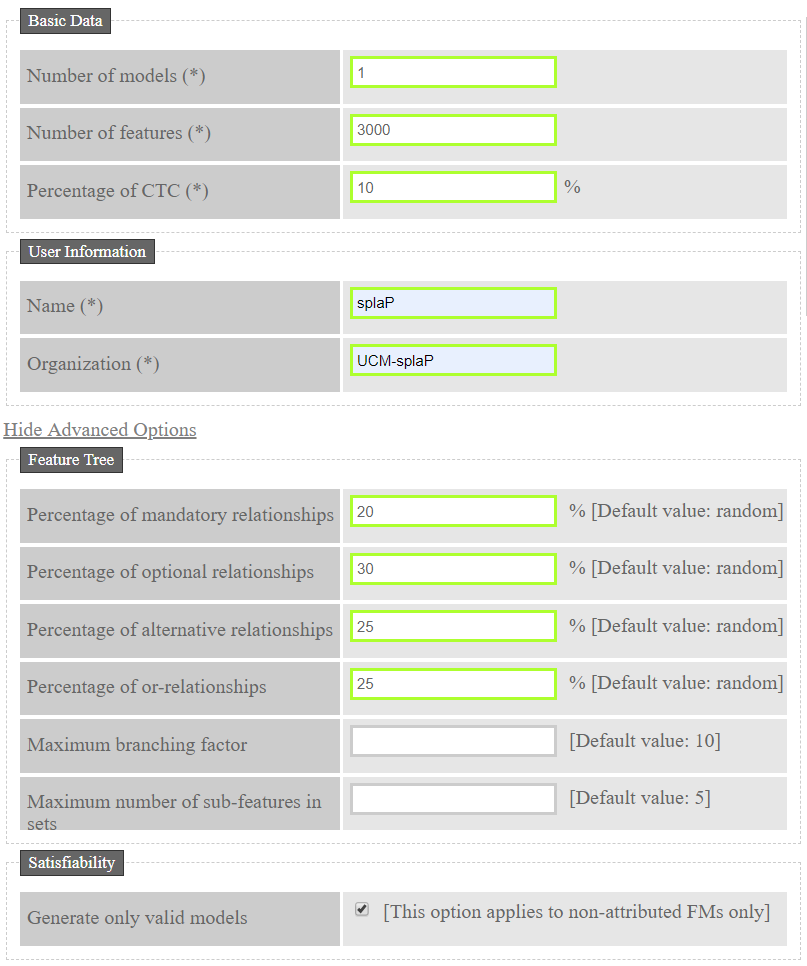
\includegraphics[width=0.8\hsize,angle=0]{BeTTy_website2.png}
        \linefigure
        \caption{BeTTy parameters.}\label{fig:plot:betty:params}
\end{figure}


BeTTy generates feature models based on a set of pre-defined parameters.
The meaning of these parameters focuses on how
BeTTy randomly generates these models.
In this case BeTTy requires 4 parameters, where the sum of the probabilities
for these parameters must be 1, that is:

\begin{itemize}
        \item The probability of having a mandatory feature.
        \item The probability of having an optional feature.
        \item The probability of having a feature in a \emph{choose-one} relationship.
        \item The probability of having a feature in a \emph{conjunction} relationship.
\end{itemize}

The values used for these parameters to generate the feature model are the following:

\begin{itemize}
        \item The probability of having a mandatory feature is 0.2.
        \item The probability of having an optional feature is 0.3.
        \item The probability of having a feature in a \emph{choose-one} relationship is 0.25.
        \item The probability of having a feature in a \emph{conjunction} relationship is 0.25.
\end{itemize}


The idea of using this configuration is to have the same probability for the different
relationships in the \fodaPAp\ term, that is, we use a probability of 0.25 for both the
\emph{choose-one} and \emph{conjunction} relationships.
%We wanted to have the same probability of having the same relationships in the model, that is
%the reason of having 0.25 for the  \emph{choose-one} and \emph{conjunction} .
Since optional features are more relevant from a probabilistic point
of view, we use a probability of 0.3 for having optional features in
the \fodaPAp\ term and a probability of 0.2 for having mandatory features.  The
sum of all probabilities must be 1. If no weight is configured, all
features and relationships have a random weight, it being not possible
to correlate the obtained results with our model analysis.
Additionally, the percentage of cross-tree constraints is set to 10\%,
which is not related to the sum of the probabilities of the previous
parameters.

\begin{figure}[h]
        \centering
        \linefigure
        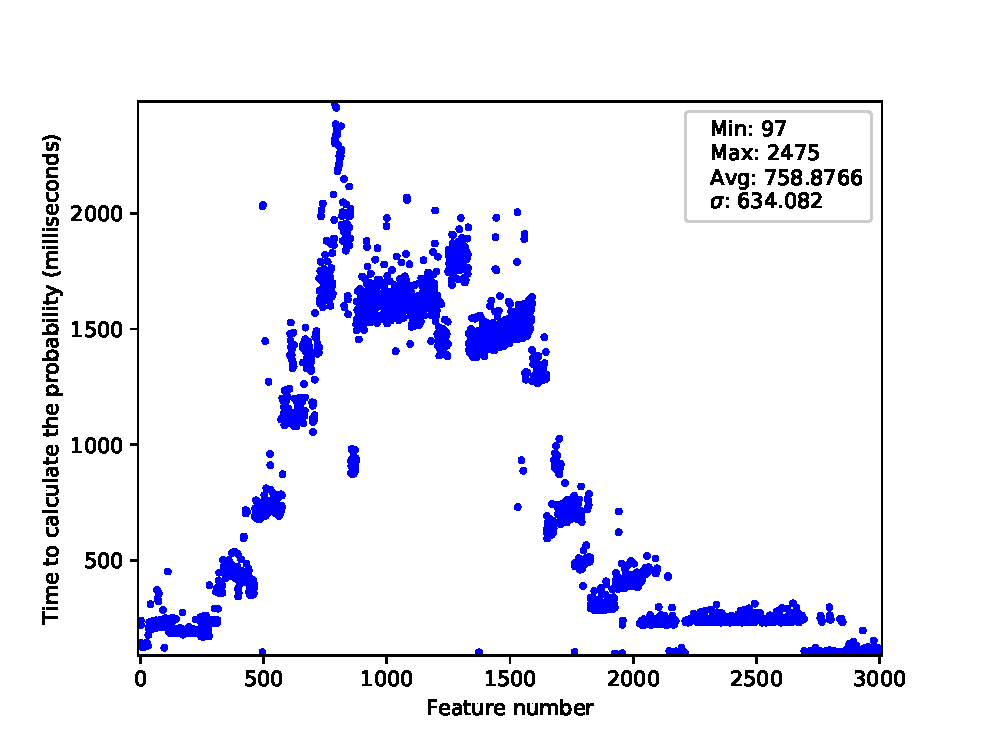
\includegraphics[width=0.8\hsize,angle=0]{plot_probs_times_FeatureModel3000.eps}
        \linefigure
        \caption{Computing time analysis for a \fodaPAp\ term consisting of 3000 features.}\label{fig:plot:probs:times}
\end{figure}

Figure~\ref{fig:plot:probs:times} shows the obtained
results from this experiment, where the x-axis depicts
the ID of each generated feature and the y-axis represents
the time required to calculate the probability of having the feature in a final product.


% It is important to remark that there is a small variation in the processing time for
% calculating the probability of each single feature. We think that this variation is
% mainly caused by both the stochastic nature of the generated model and the
% inherent noise of the node where the experiment is launched (e.g. disk latencies, operating
% system overhead, memory paging, etc.) and, therefore, it is not related to the algorithm itself.

% Since the processing time for each feature is relatively low, it being around milliseconds, a single delay in
% the process scheduling may have a direct impact in the overall algorithm performance. Hence, this overhead
% can be considered insignificant since, in general, the time for processing each feature in the model ranges
% from 15 to 28 milliseconds.

From the graphic presented in Figure~\ref{fig:plot:probs:times} we can see that giving the fact that each feature is computed independently, the
computing time to calculate its probability depends on the feature position in the \fodaPAp\ term.
Those features being lower in the model tree, will take more
time in being computed.

We have generated 11 \fodaPAp\ terms. We can observe in
Table~\ref{execution_times} that the results are similar in each
term. That is, most of  the features require between 80 and 4599 milliseconds to be processed.
% , while there is a small
% portion of them requiring a processing time between 20 and 36 milliseconds. However, there are unusual situations
% where a feature require 60 milliseconds to be processed.

\begin{table}[h]
        \centering
        \begin{tabular}{|c|c|c|c|c|}
                \hline
                \textbf{Execution} & \textbf{Minimum} &  \textbf{Maximum} &  \textbf{Average} &  \textbf{Standard deviation} \\ \hline
                \textit{1}              & 97   & 2475  & 758.8766  & 634.082        \\ \hline
                \textit{2}              & 200  & 1950  & 612.8149  & 458.745        \\ \hline
                \textit{3}              & 80   & 3201  & 895.4566  & 701.569        \\ \hline
                \textit{4}              & 350  & 4054  & 975.4781  & 700.456        \\ \hline
                \textit{5}              & 89   & 2115  & 1002.5135 & 596.598        \\ \hline
                \textit{6}              & 236  & 1800  & 490.7506  & 399.927        \\ \hline
                \textit{7}              & 409  & 2900  & 684.1667  & 650.287        \\ \hline
                \textit{8}              & 360  & 3698  & 498.3847  & 710.136        \\ \hline
                \textit{9}              & 90   & 4599  & 642.8489  & 684.993        \\ \hline
                \textit{10}             & 150  & 2700  & 870.8184  & 688.013        \\ \hline
                \textit{11}             & 84   & 2379  & 769.187   & 623.544        \\ \hline
        \end{tabular}
        \caption{Computing time analysis table.}
        \label{execution_times}
\end{table}

\begin{figure}[h]
        \centering
        \begin{minipage}[b]{0.48\textwidth}
                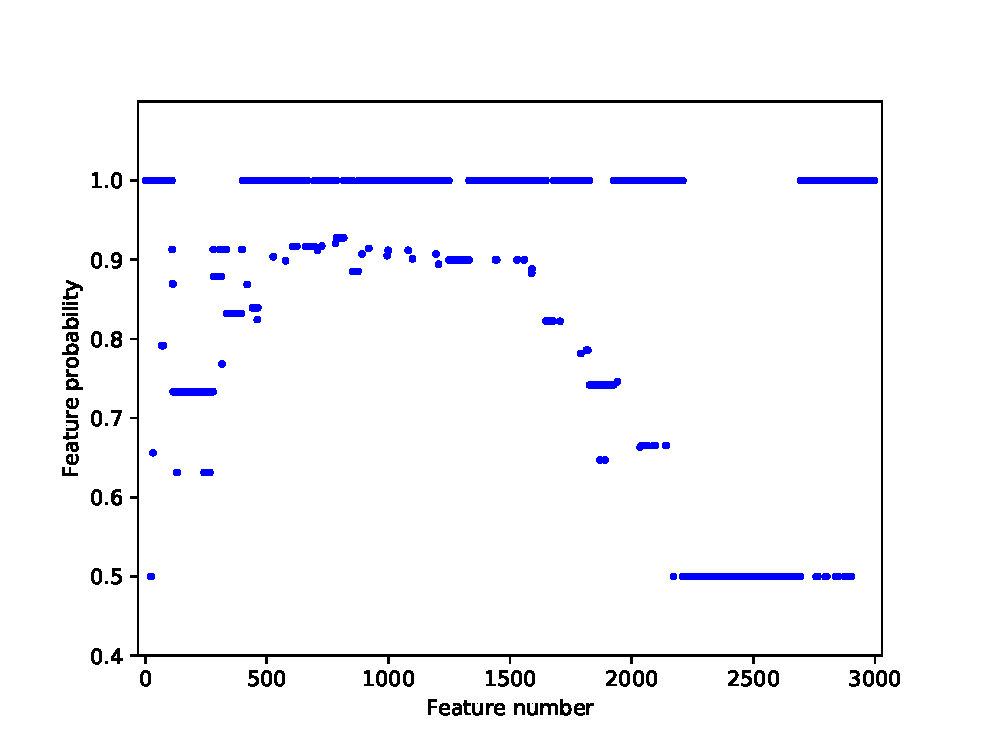
\includegraphics[width=\textwidth]{plot_probs_FeatureModel3000.eps}
\caption{Probabilistic analysis for a 3000 \fodaPAp\ term.}\label{fig:plot:probs:probs}
        \end{minipage}
        \hfill
        \begin{minipage}[b]{0.48\textwidth}
                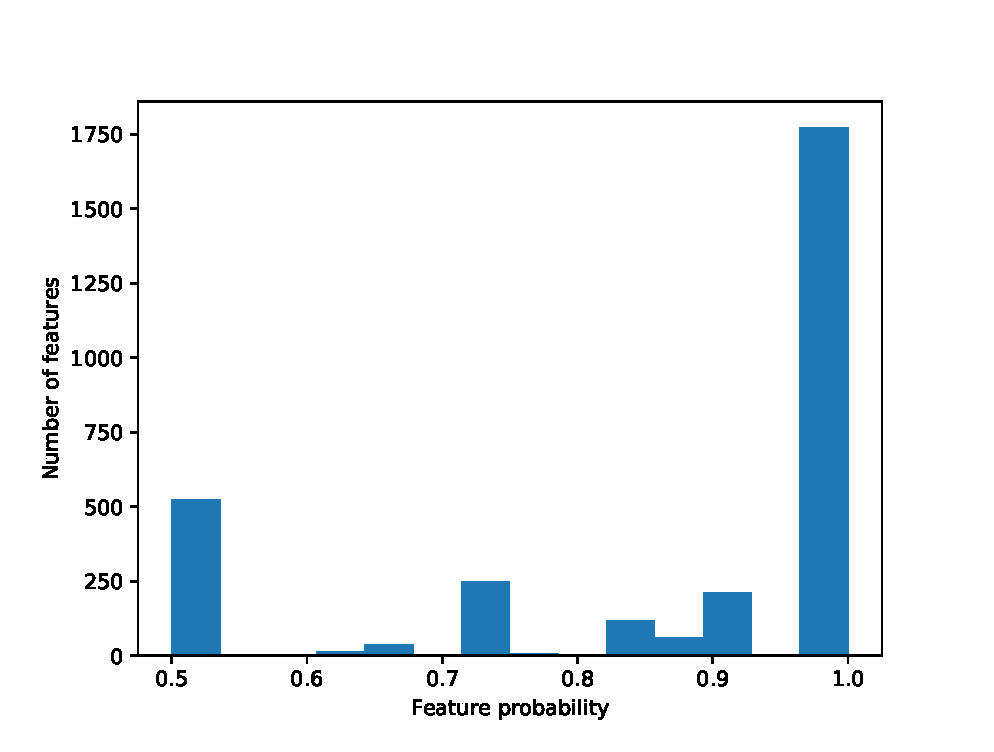
\includegraphics[width=\textwidth]{plot_probs_histogram_FeatureModel3000.eps}
        \caption{Probabilistic histogram for processing a 3000 \fodaPAp\ term.}\label{fig:plot:probs:probs:sorted}
        \end{minipage}
\end{figure}


Figure~\ref{fig:plot:probs:probs} shows the probability of each feature - in the analyzed \fodaPAp\ term - to
be part of a final product, where the $x$-axis
represents the feature ID and the $y$-axis represents the probability.
Figure~\ref{fig:plot:probs:probs:sorted} represents a histogram of the calculated probabilities for a better
readability of the results. This chart clearly shows that there exist
different groups of features having a similar probability.
In this case, the probability of the major part
of the features ranges between 0.5 and 1.
%
Thus, there are 235 features with a probability equal to 0.90 of being in a final product.
As a conclusion, this analysis might allow us to establish that by testing only
the 7.83\% of the software product line components (235 features), we can ensure that those components will be
commonly distributed in the 90\% of the products from the referenced \fodaPAp\ term.

It is important to differentiate the probabilities defined in BeTTy, which are used to generate a
\fodaPAp\ term, and the probability - calculated from the term - to have a feature in a final
product.

For instance, if we configure BeTTy to generate a \fodaPAp\ term using a probability
of 0.2 for having a mandatory feature, that means that 20\% of the generated features are mandatory.
However, that does not imply that these features be part of the 20\% of the generated products, because
the probability of having a feature in a final product depends on where this feature is placed in the
term. If a given mandatory feature is placed in a choose-one relationship, it is possible that
the other branch is used to generate the final product, discarding the mandatory feature.
Hence, we can not assume that these 20\% of the features will have a probability of 1 for being
installed in the products.

%For instance, if BeTTy is configured to generate mandatory features with a probability of 0.2 in a model, that will mean that those features will be presented in the model as mandatory with a probability of 0.2 and nothing else.
%The probability of those mandatory features in the model is not related directly with the probability of those features being part
%of let's say, the 20\% of the products, mostly, because it depends on the position of the features in the model for the
%products generation. In which case we can not assume that these 20\% of the features will have a probability of 1 for being installed
%in the products.


\subsection{Performance analysis}
\label{sec:stat:impl:performance:analysis}

Secondly, an evaluation to analyze the scalability of our approach
have been carried out. We are interested in investigating both the
execution time and the amount of memory required for processing a \fodaPAp\ term
when the number of features increases.
Hence, we use different configurations for creating a wide
spectrum of \fodaPAp\ terms, which are randomly generated,
using a different number of features that ranges from 1.000 to 10.000 (in increments of one thousand per experiment).

Specifically for each case, that is, given a configuration and a number of features,
a \fodaPAp\ term is randomly generated 30 times.
Additionally, for each term, 100 features are
randomly selected and, for each one, both the processing time and memory
required to calculate its probability are analyzed.



Table~\ref{scalaExperiment} shows the configurations used to generate the
\fodaPAp\ terms for this part of the empirical study,
where each configuration represents the set of probabilities chosen for each operator across the three experiments,
that is, \textit{Mandatory} represents the probability of having a mandatory feature,
 \textit{Optional} represents the probability of having an optional feature,
 \textit{Choose-one} represents the probability of having a feature in a \textit{choose-one} relation and
 \textit{Conjunction} represents the probability of having a feature in a \textit{conjunction} relation.

\begin{table}[h]
\centering
\begin{tabular}{|c|c|c|c|c|}
\hline
\textbf{Configuration} & \textbf{Mandatory} &  \textbf{Optional} &  \textbf{Choose-one} &  \textbf{Conjunction} \\ \hline
        \textit{1}              & 0.69  & 0.15  & 0.15  & 0.01  \\ \hline
        \textit{2}              & 0.5           & 0.15  & 0.15  & 0.2           \\ \hline
        \textit{3}              & 0.2           & 0.15  & 0.15  & 0.5   \\ \hline
\end{tabular}
\caption{Configuration of the scalability experiments.}
\label{scalaExperiment}
\end{table}

In this experiment, we have set the same values for the probabilities of the \textit{Optional}
and \textit{Choose-one} features. Hence, these will remain the same
across all the experiments and, thus, they should not interfere in the obtained results.
We start with a low probability of having a \textit{Conjunction} relationship in the \fodaPAp\ term. In this
case, for the first experiment, we use a probability of 0.01, which is increased in the next configurations
to 0.2 and 0.5, respectively. This idea is to show the impact of the \textit{Conjunction} relationship in the time
and memory required for processing the \fodaPAp\ terms.

For each configuration, we have generated 30 \fodaPAp\ terms per number of features, that is, we generate
30 different \fodaPAp\ terms containing 1000 features, 30 different \fodaPAp\ terms containing 2000 features,
and so on until 10.000 features.

Figure~\ref{fig:plot:probs:boxplot_0_1} and figure~\ref{fig:plot:probs:boxplot_0_1_mem}
show the execution time and the required amount of memory, respectively, for processing
the \fodaPAp\ terms generated using \textit{Configuration 1}. In these terms, only 1\% of
the features have a conjunction relation. In general, the processing time when the number
of features increases is linear. Only in few cases, where the number of features ranges
from 5000 to 8000, the results provide anomalous values. This is mainly caused by the
random nature of the generated terms (30 for each case). On the contrary, the memory
usage depicts that there are several groups where the memory usage remains constant,
one group of terms containing between 3,000 and 5,000 features and other group of terms
containing between 7,000 and 10,000 features. In summary, our implementation shows good
scalability results for processing the terms generated using \textit{Configuration 1}:
it requires, in the worst case scenario, 215 ms and 0.32 GB of RAM to process the terms.

\begin{figure}[h]
        \centering
        \begin{minipage}[b]{0.48\textwidth}
                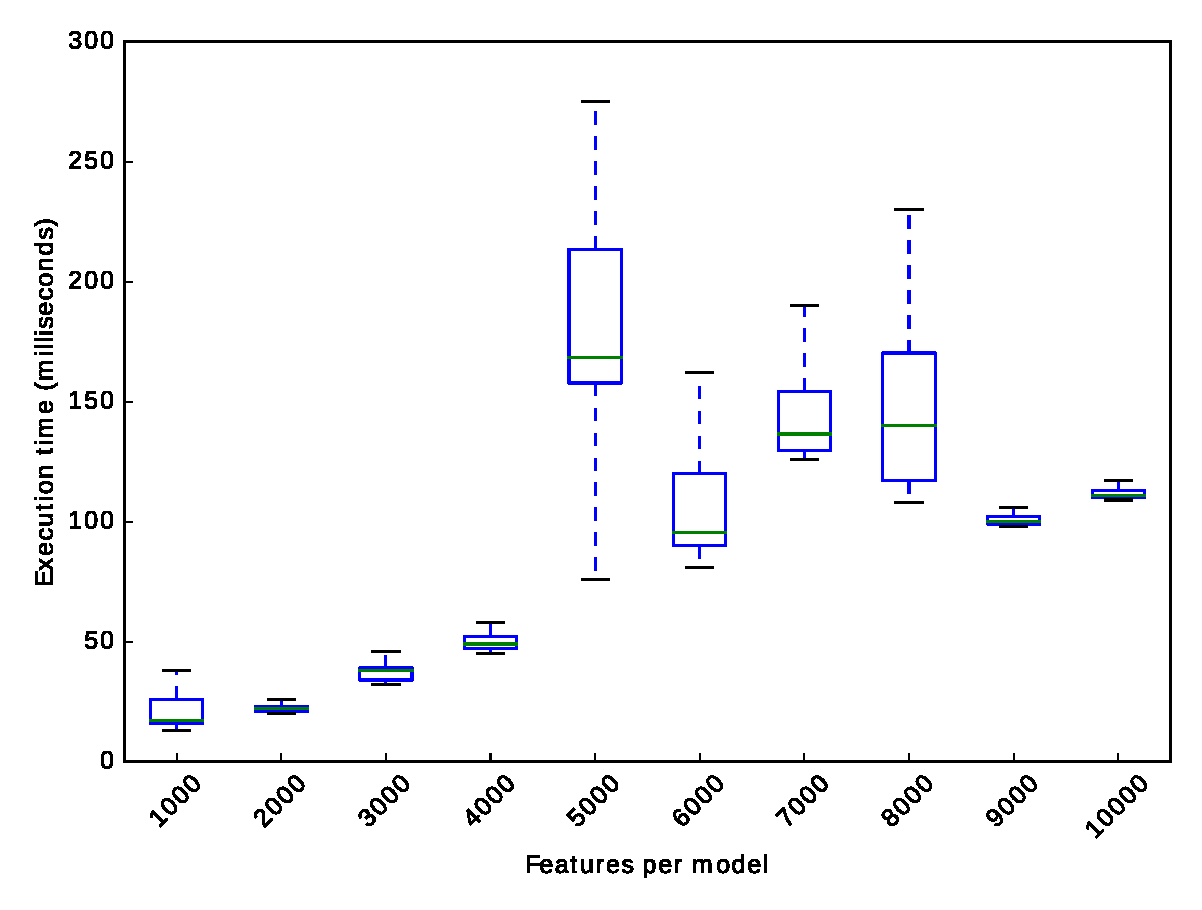
\includegraphics[width=\textwidth]{boxplot_0_1.eps}
                \caption{Execution time for processing the \fodaPAp\ terms generated using \textit{Configuration 1}.}\label{fig:plot:probs:boxplot_0_1}
        \end{minipage}
        \hfill
        \begin{minipage}[b]{0.48\textwidth}
                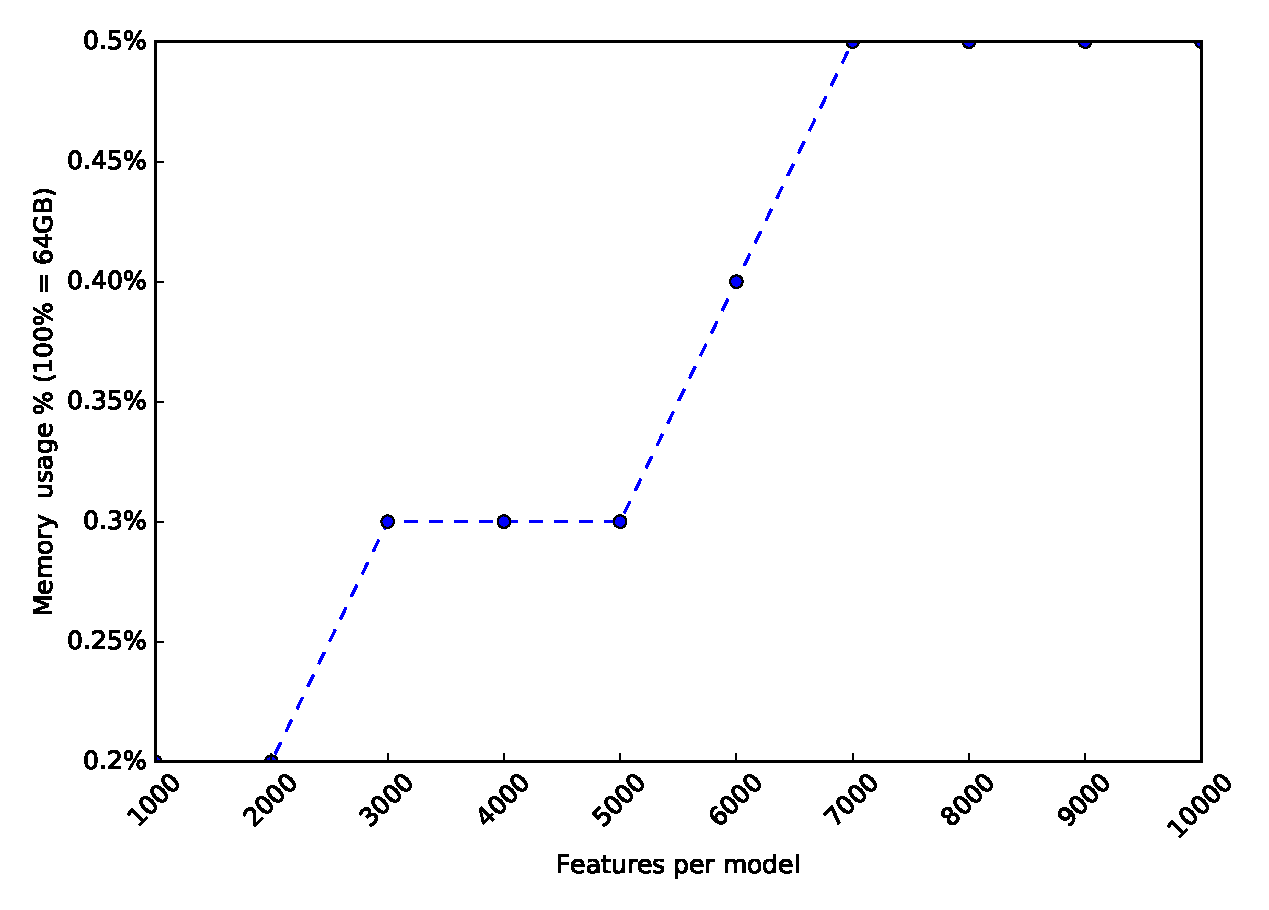
\includegraphics[width=\textwidth]{boxplot_0_1_mem.eps}
                \caption{Memory usage for processing the \fodaPAp\ terms generated using \textit{Configuration 1}.}\label{fig:plot:probs:boxplot_0_1_mem}
        \end{minipage}
\end{figure}

Figure~\ref{fig:plot:probs:boxplot_0_2} and figure~\ref{fig:plot:probs:boxplot_0_2_mem} show
the results for analyzing the generated terms using \textit{Configuration 2}. It is important
to remark that 20\% of the features in the generated terms have a conjunction relation. In this
case, both the execution time and memory usage for processing a term when the number of features
increases are exponential. These charts clearly show a turning point when the term reaches 6,000
features and, therefore, the required processing time and  memory are significantly lower for those
terms that do not reach 6,000 features. However, the requirements to process the term in the worst
case scenario, that is, using a term containing 10,000 features, are 300 sec. and 3.84 GB of RAM memory,
which are acceptable.

\begin{figure}[h]
        \centering
        \begin{minipage}[b]{0.48\textwidth}
                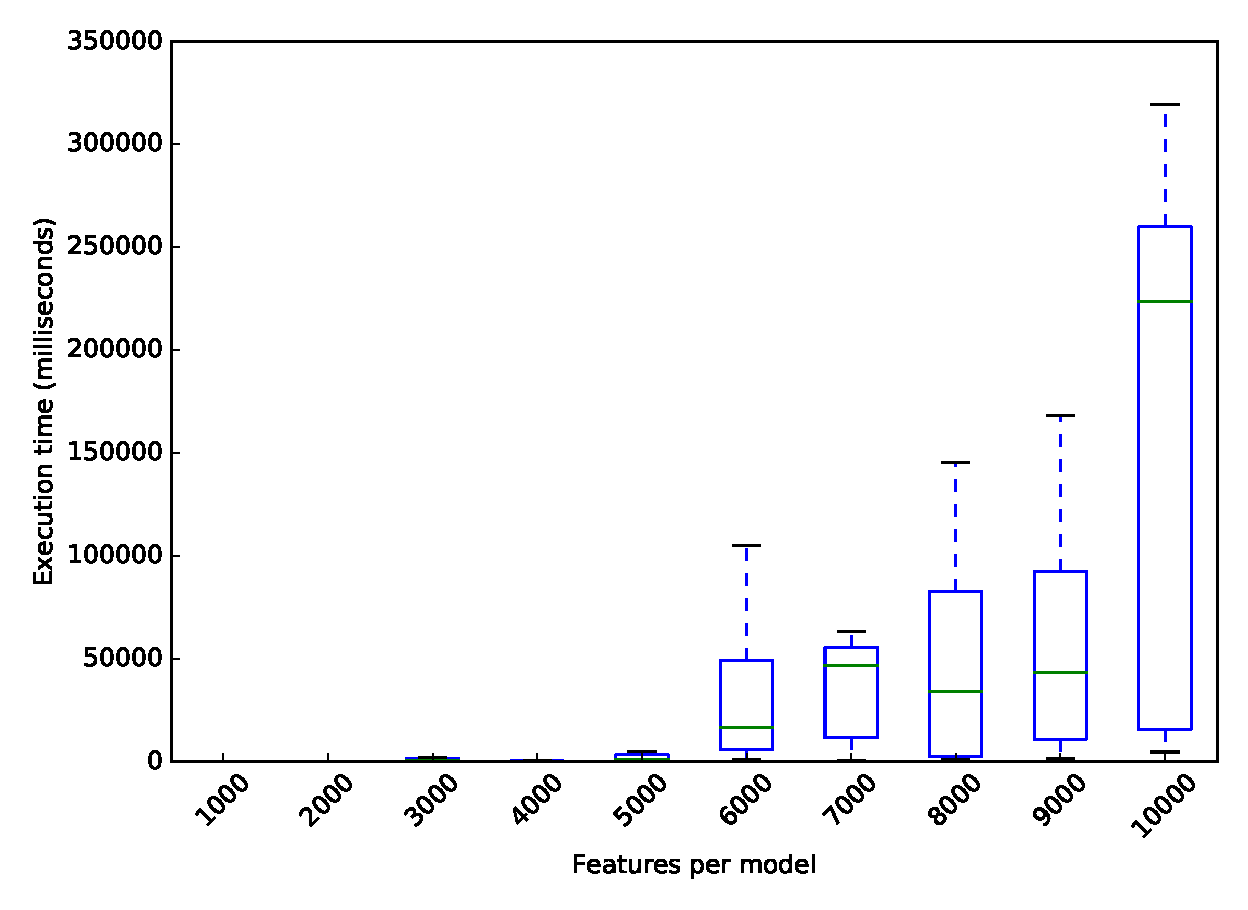
\includegraphics[width=\textwidth]{boxplot_0_2.eps}
                \caption{Execution time for processing \fodaPAp\ terms generated using \textit{Configuration 2}.}\label{fig:plot:probs:boxplot_0_2}
        \end{minipage}
        \hfill
        \begin{minipage}[b]{0.48\textwidth}
                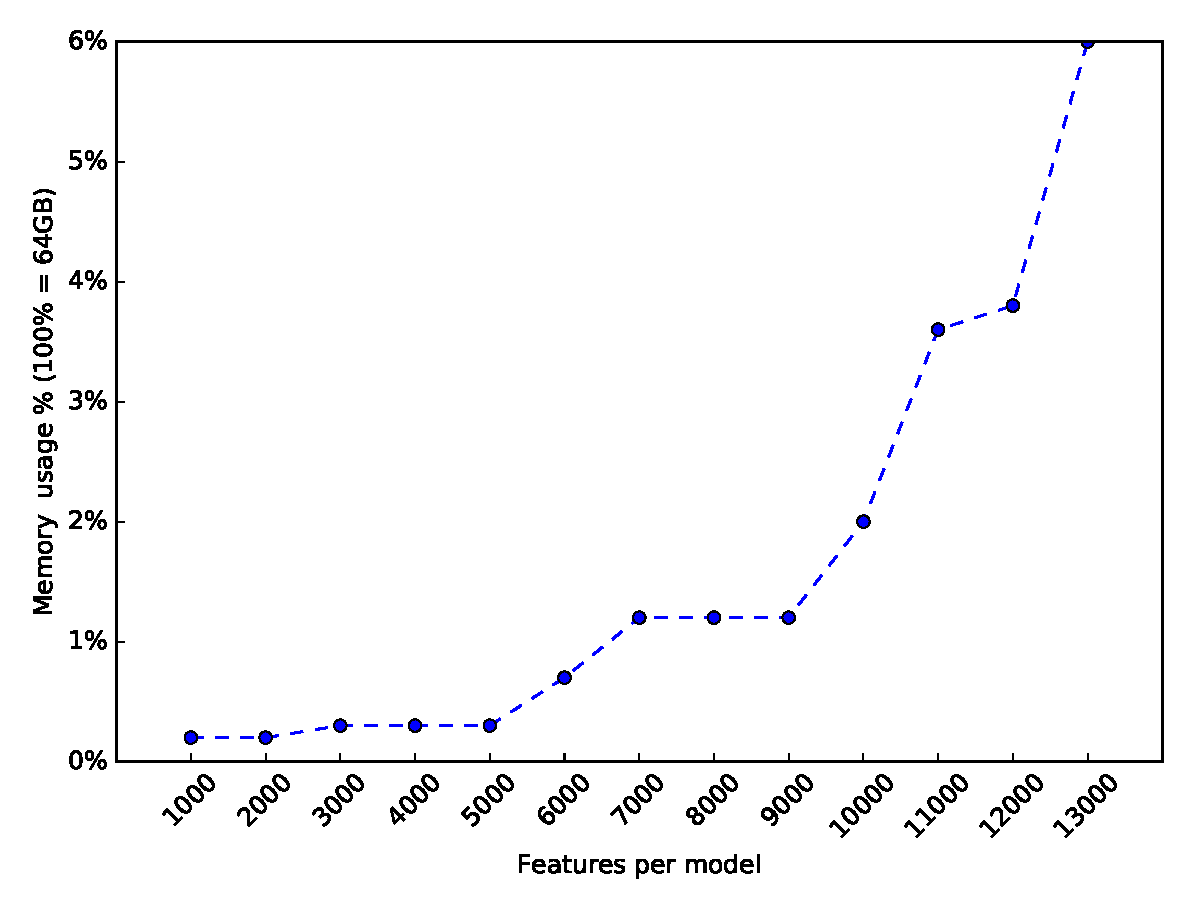
\includegraphics[width=\textwidth]{boxplot_mem.eps}
                \caption{Memory usage for processing \fodaPAp\ terms generated using \textit{Configuration 2}.}\label{fig:plot:probs:boxplot_0_2_mem}
        \end{minipage}
\end{figure}

Figure~\ref{fig:plot:probs:boxplot_0_5} and figure~\ref{fig:plot:probs:boxplot_0_5_mem} show
the results for processing the terms generated using \textit{Configuration 3}. In this case,
half of the features in the term have a conjunction relation. Similarly to the previous experiment,
these charts show that both the execution time and the memory usage for processing a term when the
number of features increases are exponential. In the obtained results we can observe the same
turning point detected in the previous terms generated using  \textit{Configuration 2}, that is,
when the term reaches 6,000 features. Terms processing requirements, that is, execution time and
memory usage, grow much faster for these terms than for those based on previous configurations.
Also, it is important to notice that the terms containing 9,000 and 10,000 features cannot be
processed due to memory limitations.

\begin{figure}[h]
        \centering
        \begin{minipage}[b]{0.48\textwidth}
                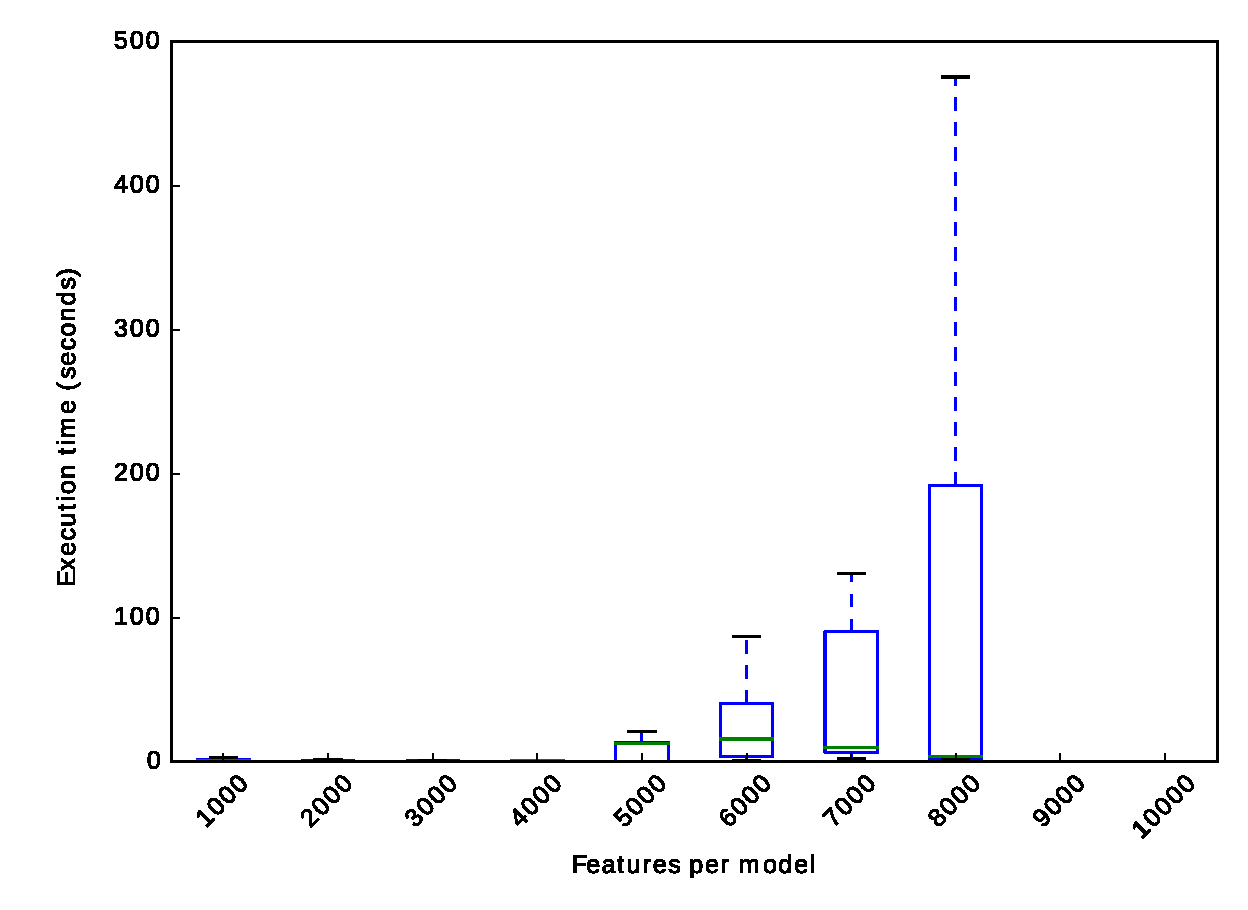
\includegraphics[width=\textwidth]{boxplot_0_5.eps}
                \caption{Execution time for processing \fodaPAp\ terms generated using \textit{configuration 3}.}\label{fig:plot:probs:boxplot_0_5}
        \end{minipage}
        \hfill
        \begin{minipage}[b]{0.48\textwidth}
                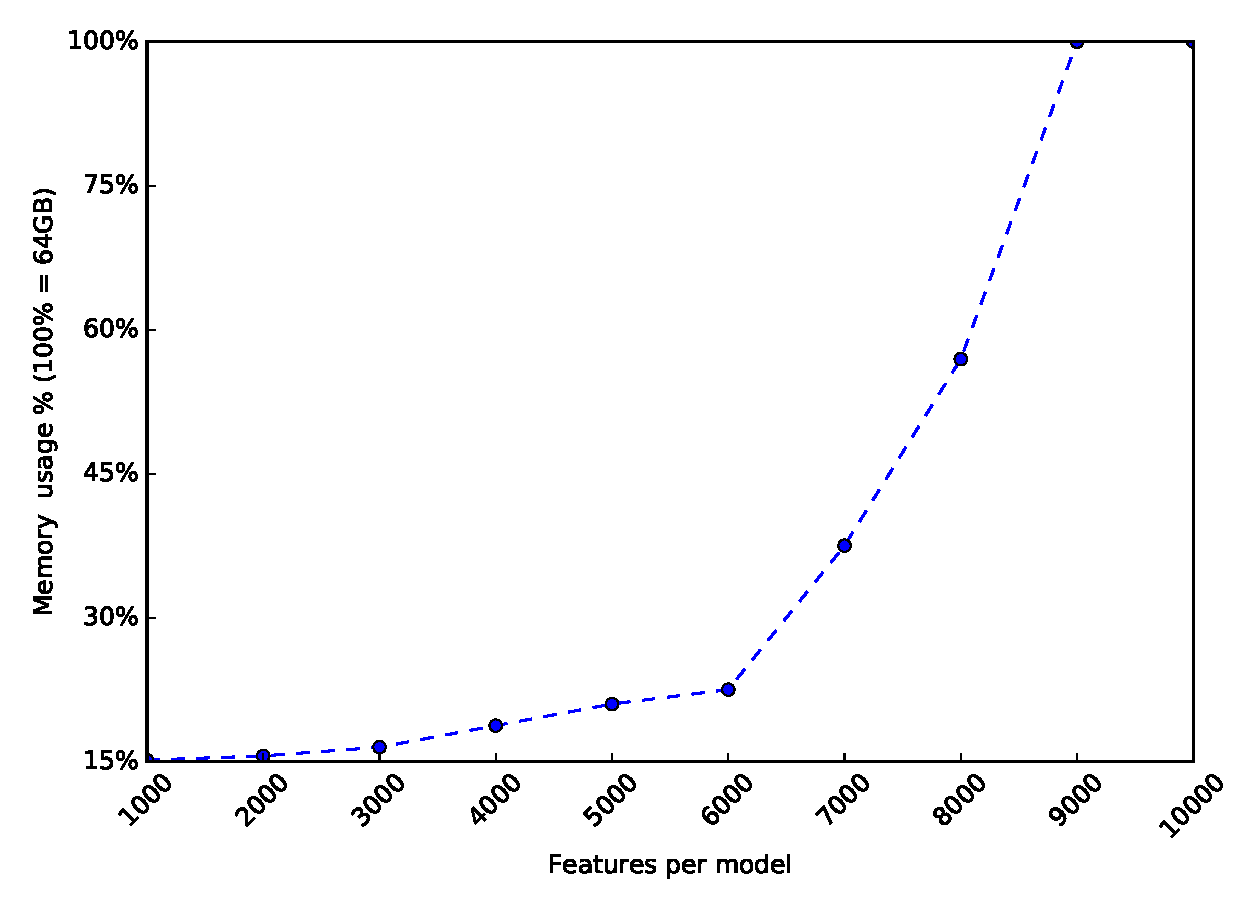
\includegraphics[width=\textwidth]{boxplot_0_5_mem.eps}
                \caption{Memory usage for processing \fodaPAp\ terms generated using \textit{configuration 3}.}\label{fig:plot:probs:boxplot_0_5_mem}
        \end{minipage}
\end{figure}


%%%------------------------------------------------------------------------------------------------------------------------------------------------

\subsection{Discussion of the results}
\label{sec:stat:impl:comp}

In this section we discuss the results obtained from the empirical study. Specifically,
we are interested in analyzing the performance of the implementation of the probabilistic
extension. Also, we provide the answers for the research questions.

The experiments carried out in Section~\ref{sec:stat:impl:performance:analysis}
uses \fodaPAp\ terms containing a maximum of 10000 features. In general,
these results show that increasing the number of features having a conjunction relation
has a direct impact on the overall performance. In fact, increasing the number of features having
a conjunction relation generates a combinatorial explosion that hampers the processing of the \fodaPAp\ terms.
First, the execution time to completely process a term significantly grows. Second, large amounts
of memory are required to store those combinations. In some cases, using large terms with a high
percentage of features having a conjunction relation may cause a bottleneck in the memory system.
In fact, terms generated using \textit{Configuration 3} with 9,000 and 10,000 features cannot be
processed using 64 GB of RAM. In this case,
the worst case scenario, which generates a \fodaPAp\ term where the 50\% of the features are
placed in a conjunction relationship, requires approximately 500 seconds.

%Figure~\ref{figure:tool:den:benchmark} shows the results of an experiment using
%models containing different number of features, which ranges from $50$ to $300$.
%In this case, we use the implementation of the denotational semantic from
%\fodaPA~\cite{acl13} to process the models, which do not use probabilistic
%information. If we use only the executions that successfully process the model,
%the worst case scenario requires 786.126 seconds to process a model containing 150
%features. Additionally, Figure~\ref{fig:cluster} shows the results published in
%\fodaPAc~\cite{clc16}, where the models used for the simulations were processed in
%an 8-node cluster. In this case, the generated models only contain 17 features and
%the best time for processing the model is approximately 300 seconds.
%
%\begin{figure}[t]
%        \centering
%        \begin{minipage}{0.4\hsize}
%        \begin{tabular}{|rrr|}
%                        \hline
%                Features&       Time (ms.)&    Products\\
%                        \hline
%                50 & 6 & 48 \\
%                60 & 25 & 108 \\
%                70 & 15 & 104 \\
%                80 & 8 & 31 \\
%                90 & 38 & 0 \\
%                100 & 55 & 1404 \\
%                110 & 13 & 12 \\
%                120 & 2139 & 1 \\
%                130 & 511 & 24802 \\
%                140 & 7 & 6 \\
%                150 & 786126 & 1312848 \\
%                160 & 136 & 5670 \\
%                170 & 42 & 398 \\
%                \hline
%        \end{tabular}
%        \end{minipage}
%        \begin{minipage}{0.4\hsize}
%        \begin{tabular}{|rrr|}
%                \hline
%                Features&       Time (ms.)&    Products\\
%                        \hline
%180 & 744 & 6384 \\
%190 & 1390 & 7232 \\
%200 & 960000 & - \\
%210 & 97770 & 800544 \\
%220 & 263 & 51 \\
%230 & 47 & 8 \\
%240 & 65 & 29 \\
%250 & 191 & 5920 \\
%260 & 205 & 7296 \\
%270 & 250 & 4301 \\
%280 & 960000 & - \\
%290 & 65 & 3 \\
%300 & 960000 & - \\
%                \hline
%        \end{tabular}
%        \end{minipage}
%        \caption{Denotational benchmark from \cite{acl13}.\label{figure:tool:den:benchmark}}
%\end{figure}
%
%
%\begin{figure}[t]
%        \centering
%        \linefigure
%        \resizebox{\columnwidth}{!}{%
%                \begin{tabular}{|c|c|c|c|c|c|c|}
%                        \cline{2-7}
%                        \multicolumn{1}{c|}{} & 1 Worker & 2 Workers & 4 Workers & 8 Workers & 16 Workers & 32 Workers  \\
%                        \hline
%                        1 Node & 2010.44763303 & 1060.80047798 & 586.014445066 & 543.712262154 & 521.616870165 & 521.292215109 \\
%                        \hline
%                        2 Nodes & 2059.06947899 & 1046.87119007 & 575.115453959 & 296.285589933 & 366.384442091 & 341.007520199 \\
%                        \hline
%                        4 Nodes & 2031.25184584 & 1093.52087283 & 586.344302893 & 320.010899067 & 300.745616913 & 382.748430014 \\
%                        \hline
%                        8 Nodes & 2207.35427213 & 1143.951792 & 576.370896101 & 495.507214785 & 308.374300957 & 287.340030909 \\
%                        \hline
%                \end{tabular}
%        }\\
%        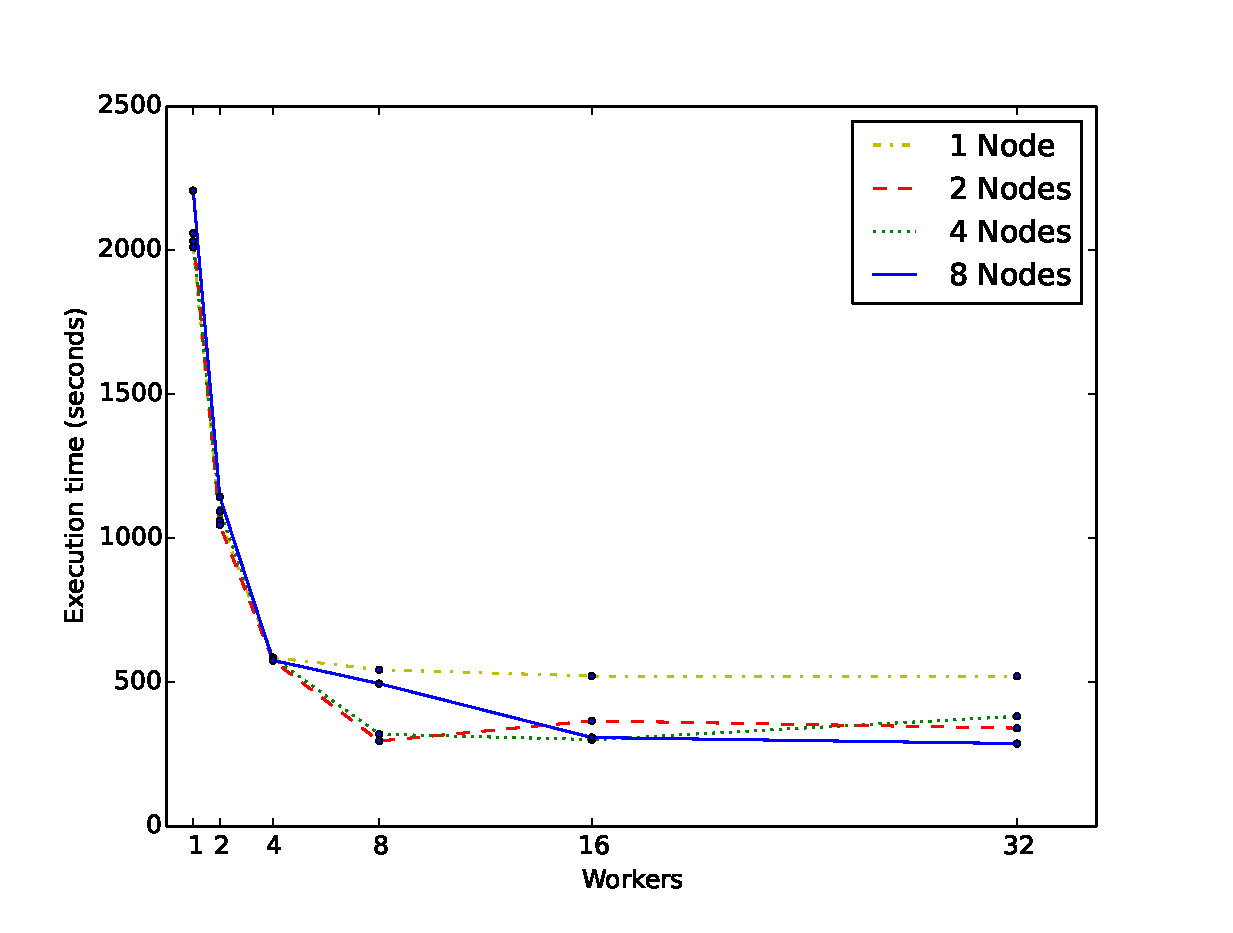
\includegraphics[width=0.7\hsize, height=5cm,angle=0]{plot_cluster.eps}
%        \linefigure
%        \caption{Cluster execution times for 1, 2, 4 and 8 nodes; and 1, 2, 4, 8, 16 and 32 workers  from~\cite{clc16}.}\label{fig:cluster}
%\end{figure}
%
%It is important to remark that the number of features of the models generated in
%these previous works is considerably lower than the number of features of the models
%used in this empirical study. Since algorithms developed in~\cite{acl13,clc16} require a
%high computational power to process the models,
%it was unfeasible to use models containing thousands of features. Consequently, in this case,
%the obtained results show that the performance of the denotational semantics of the
%probabilistic extension implementation allows to process larger models more efficiently than
%the denotational semantics implementations presented in previous works~\cite{acl13,clc16}.

Following, we provide the answers to the research questions.

\textbf{RQ1}: Is it possible to translate current graphical representations of feature models to
support probabilistic information?


In order to answer this question we have implemented the denotational semantic
of the probabilistic extension. Since our framework is based on \FODA, we
can state that the answer is yes, it is possible to translate current graphical
representations of feature models, like \FODA, to represent and support probabilistic
information.

\textbf{RQ2}: Is it possible to extend \fodaPA\ in such a way that
translates the probabilistic information from the graphical representation to a formal representation?

General use models have been proposed to model variability in software
product lines~\cite{tlll15, tllv15} and, specifically, for feature-oriented
systems~\cite{Dubslaff2015, Chrszon2018}.
Thus, all previous work focuses on
generic representations. However, this work is based on including probabilistic
information to the well-known feature model \FODA.
Based on our previous results~\cite{acl13,clc16}, together with the results
presented in this work, we can state that state it is possible to
describe a formal framework that translates the current graphical
definitions of feature models into to a probabilistic formal representation.

\textbf{RQ3}: What is the impact of applying probabilistic analysis methods
to current feature models like \FODA?

In order to answer this question we carried out some experiments using
our implementation of the probabilistic extension. Since the probabilistic extension
focuses on hiding  those features that do not affect the processing of the
probability of given feature for being part of a valid product, the required
time for processing the \fodaPAp\ term is considerably reduced. Hence, the
implementation of the probabilistic extension provides a greater scalability
than our previous implementations of the denotational semantic \fodaPA~\cite{acl13}
and the cost extension \fodaPAc~\cite{clc16} and, therefore, large terms containing
an elevated number of features are processed more efficiently. Although these
previous implementations also allow to calculate all the valid products of a term, the
required processing time to accomplish this task is elevated, making the
processing of large terms unfeasible. Alternatively, the implementation of the denotational
semantic \fodaPA~\cite{acl13} also calculates the satisfactibility of a
term, that is, checks if the term contains, at least, a valid product. In this case,
this implementation requires less computing time at the cost of providing a simpler
simpler result, which contains less information than the one generated
by the probabilistic extension.

%In order to answer this question we carried out some experiments using
%our implementation of the denotational semantic \fodaPA~\cite{acl13}
%and the cost extension \fodaPAc~\cite{clc16}. The results obtained
%have been compared with the implementation of the probabilistic
%extension. We observed that the latter is able to process larger
%models faster, which provides a greater scalability when
%the size of the model to be processed grows.


%\begin{figure}[t]
%$$
%\begin{array}{ccc}
%\mathtt{Test}&\mathtt{Features}& \mathtt{Time}\\
%\#1& \feature{A},\feature{B} & 10\ units\\
%\#2& \feature{C},\feature{D} & 15\ units\\
%\#3& \feature{A},\feature{C},\feature{D} & 8\ units\\
%\#4& \feature{C},\feature{B} & 9\ units\\
%\end{array}
%$$
%\caption{Input parameter: test suite\label{fig:input:parameter}}
%\end{figure}

%We have two open issues:
%\begin{description}
%\item[Unit testing]  Let $P$ be a software product line, and $T_{unit}$ be a
%  test suite. Each test checks the correctness of a feature (i.e, %\feature{A} or \feature{B}).
%  We can compute the \emph{probability} of a feature. We test before those features with bigger probability.
%  \begin{itemize}
%  \item We can calculate the most frequent set of features in $P$ to test.
  %\item  We can provide a coverage of the test suite taking into account the percentage of appearance of each feature.
  %\end{itemize}

%\item[Integration testing] We have a test suite $T_{integration}$ where each test checks
%  the integration of a product.
%  Let us note that the integration of the product $\{\feature{A},\feature{B}\}$  can be different than
%  the integration of $\{\feature{A}, \feature{B},\feature{C}\}$.
%  \begin{itemize}
%  \item Which tests of the suite can be applied in this SPL?
 % \item What is the coverage of each test suite?
 % \end{itemize}


%\end{description}


%Next step is to associate to each integration test the time that
%it needs to be completed.
%For instance in Figure~\ref{fig:input:parameter} we represent some integration tests and the
%time that they need to be completed.



%\begin{quote}
%\emph{Let us consider an integration test suite and a probabilistic SPL $P$.
%If we only have $n$ time units, which is the \emph{best set} of tests
%to check the correctness of $P$? We say that a test is better than another
%test if its representativity (the probability to perform these features together) is higher.}
%\end{quote}

%\bprop
%        The previous problem is NP-hard\ccomen{I propose the transformation into the Subset Sum problem.}.
%\eprop

%Next we define the subset sum problem.

%\bdfn
%    Let $A = \{a_1, a_2, \ldots, a_n\}$ be a  set of natural numbers and $s$ be  a positive integer.
%    The subset sum problem checks if there is a subset $A'\subseteq A$ such that:  $$\sum_{a\in A'} = s$$
%\edfn

%In our previous problem we have a set of pairs $B=\{(p_{1},t_{1}),(p_{2},t_{2}),\ldots,(p_{n},t_{n})\}$ where
%$p_{i}$ is the probability to perform the test $i$ and $t_{i}$ is the time needed to perform this test, and
%two constants $P$ and $T$. $P$ will represent a probability value and $T$ a time value.
%We are looking for those pairs $(p_{i},t_{i}),\ldots,(p_{j},t_{j})\in B$ that
%$$
%\begin{array}{ll}
%p_{i}+\ldots +p_{j} &\geq P\\
%t_{i}+\ldots +t_{j} &\leq T\\
%\end{array}
%$$

%Let us consider that $p_{i}=t_{i}={a_i}$ and $P=T=s$.
%We can rewrite the previous problem into

%$$
%\left.
%\begin{array}{ll}
%a_{i}+\ldots +a_{j} &\geq s\\
%a_{i}+\ldots +a_{j} &\leq s\\
%\end{array}
%\right\}=
%a_{i}+\ldots +a_{j} = s\
%$$

%And we have the subset sum problem\ccomen{Please check because $p_{i}$ and $t_{i}$ can be reals while $s_{i}$ are integers}.


%\begin{enumerate}
%        \item We can create a GA to solve this problem.
%        \item We have that this problem is FPTAS~\cite{Ibarra:1975:FAA:321906.321909}.
%\end{enumerate}



%In order to obtain a set of tests that holds the previous issues, we propose
%two implementations.
%The first one is using a dynamic algorithm while the second one to use a genetic algorithm.

%\subsection{Dynamic algorithm}

% We adapted the dynamic algorithm of 0-1 Knapsack problem
%to our problem and we implemented it in python.


%We define a matrix $A$, where $A(i,j)$ contains the
%maximum value that can be attained from considering
%only the sum of the first i tests' probability that need at most j time units.


%$$
%A(i,j)=
%\left\{
%        \begin{array}{lll}
%        0 &\hspace*{3em}&\si i=0 \lor j = 0\\
%        A(i-1,j) & & \si t_i>j\\
%        \max{(A(i-1,j),p_{i}+A(i-1,j-t_i))} &&\si t_i \leq j
%        \end{array}
%\right.
%$$

%In our case, we will say that $A(n,T)$ is the solution if the sum of the  percentages
%of all elements involved in this solution is bigger than or equal to $P$. Otherwise we do not have a solution.


%For instance, in Table~\ref{figure:input:parameters} there are presented a set of 24
%different tests with their time consuming and its probability.
%For instance the first element, t1,9,150, means the test t1 needs 9 time units to be completed
%and the value associated with this test is 150\footnote{We could put here a measure, the probability or anything}.

%\begin{table}
%\centering

%\selectfont
%{\tt
%\begin{tabular}{|l|l|l|}
%\hline
%\#1,9,150 &
%\#2,13,35&
%\#3,153,200\\
%\#4,50,160&
%\#5,15,60&
%\#6,68,45\\
%\#7,27,60&
%\#8,39,40&
%\#9,23,30\\
%\#10,52,10&
%\#11,11,70&
%\#12,32,30\\
%\#13,24,15&
%\#14,48,10&
%\#15,73,40\\
%\#16,42,70&
%\#17,43,75&
%\#18,22,80\\
%\#19,7,20&
%\#20,18,12&
%\#21,4,50\\
%\#22,30,10&
%\#23,90,1&
%\#24,200,150\\
%\hline
%\end{tabular}}
%\caption{Input parameter (test,time,value) for the test selection algorithm.\label{figure:input:parameters}}
%\end{table}

% \begin{figure}[t]
% \centering
% includegraphics[scale=1]{GA_Flowchart_4}
% \caption{Scheme of GA.\label{scheme:genetic:algorithm}}
% \end{figure}





% After executing the dynamic algorithm, with the following input parameters a)
% the data presented in Table~\ref{figure:input:parameters} and T (the maximum time value) equals to 500,
% we obtain that {\tt \#1, \#2, \#3, \#4, \#5,
% \#7, \#8, \#9, \#11, \#12, \#16, \#17,
% \#18, \#19} and {\tt \#21}       conforms the final solution, and P =  1130.


% \subsection{Genetic Algorithm}

% Next we perform a genetic algorithm to discover a better solution.
% The GA structure is in Figure~\ref{scheme:genetic:algorithm}.
% With this algorithm we obtain values bigger than 1130.






% \subsubsection{Representation}
% We represent the possible solutions (those tests that hold the conditions) as follows:
% \begin{itemize}
%         \item Genotype: Given $n$ tests, we represent a solution with a binary (1/0) string
% of length $n$ where the position i determines whether the ith-test is included or not.
% The genotype space is complete, that is, any valid solution can be mapped in this array.
%         \item Phenotype: There are only some genotypes that are \emph{correct}. These are
% those that taking the $n'$, with $n'\leq n$ first $1$ bits from left to right of a genotype, we have that the sum of
% the time values associated with these tests is lower than or equal to T,
% and that the representativity of these tests is $\geq P$.
% \end{itemize}


% \subsubsection{Initial Population}
% We execute the algorithm with the parameters presented in Figure~\ref{fig:parameters:initial:population} in order to show
% how many initial population do we need.
% There is an interesting effect that this experiment reveals.
% The first and second graphs indicate that for populations smaller than 50 the chance for premature convergence seems to be rather high.
% Therefore we will consider that a good candidate for initial population is 500.

% \begin{figure}[t]
% \centering

% \begin{minipage}{0.45\hsize}\centering
%         \textbf{x}=10

% \includegraphics[scale=0.3]{graphs_basea/basea_diff_raw}
% \end{minipage}
% \begin{minipage}{0.4\hsize}\centering

%         \textbf{x}=50
% \includegraphics[scale=0.3]{graphs_baseb/baseb_diff_raw}

% \end{minipage}


% \begin{minipage}{0.45\hsize}\centering
%         \textbf{x}=200

% \includegraphics[scale=0.3]{graphs_based/based_diff_raw}
% \end{minipage}
% \begin{minipage}{0.4\hsize}\centering

%         \textbf{x}=500
% \includegraphics[scale=0.3]{graphs_basec/basec_diff_raw}

% \end{minipage}

% {\centering
% %\fontsize{7}{9}
% %\selectfont

% \begin{tabular}{|l|l|}
% \hline
% Representation  &Binary strings of length n\\
% Recombination   &One point crossover\\
% Recombination probability &     80\\
% Mutation        & Swap Mutator \\
% Mutation probability    & 2\% \\
% Parent selection        & Roulette\\
% Survivor selection      & Generational\\
% Population size         & \textbf{x} \\
% Termination condition   & Terminate the evolution based on the fitness stats\\
% Generations     & 100 \\
% \hline
% \end{tabular}}

% \caption{Comparing initial population\label{fig:parameters:initial:population}.}
% \end{figure}



% \subsubsection{Recombination probability}
% Next we study the effect of changing the recombination probability.
% In Figure~\ref{fig:parameters:recombination} we show the max fitness, average fitness and
% minimum fitness of the population, in each generation, using the probability values 0.1, 0.4, 0.8 and 1 for recombination.
% We will use 0.8 in the rest of experiments because a) we obtain the maximum fitness, and b) the difference between maximum and minimum is low.

% Let us also note that adding more values of recombination probability (i.e, 100\%), that is also presented in
%  Figure~\ref{fig:parameters:recombination} does not imply to have better fitness solutions. So, this value should be high
% but not 100\%.

% \begin{figure}[t]

% \centering

% \begin{minipage}{0.5\hsize}\centering
%         \textbf{x}=0.1

% \includegraphics[scale=0.3]{graphs_basee/basee_maxmin_fitness}
% \end{minipage}
% \begin{minipage}{0.4\hsize}\centering

%         \textbf{x}=0.4
% \includegraphics[scale=0.3]{graphs_basef/basef_maxmin_fitness}

% \end{minipage}


% \begin{minipage}{0.50\hsize}\centering
%         \textbf{x}=0.8

% \includegraphics[scale=0.3]{graphs_baseg/baseg_maxmin_fitness}
% \end{minipage}
% \begin{minipage}{0.4\hsize}\centering

%         \textbf{x}=1
% \includegraphics[scale=0.3]{graphs_baseh/baseh_maxmin_fitness}

% \end{minipage}


% {\centering
% %\fontsize{7}{9}
% %\selectfont

% \begin{tabular}{|l|l|}
% \hline
% Representation  &Binary strings of length n\\
% Recombination   &One point crossover\\
% Recombination probability &     \textbf{x}\\
% Mutation        & Swap Mutator \\
% Mutation probability    & 2\% \\
% Parent selection        & Roulette\\
% Survivor selection      & Generational\\
% Population size         & 500 \\
% Termination condition   & Terminate the evolution based on the fitness stats\\
% Generations     & 100 \\
% \hline
% \end{tabular}}

% \caption{Comparing recombination probability\label{fig:parameters:recombination}.}
% \end{figure}

% \subsubsection{Mutation operator}

% We define two mutation operators in the chromosomes. The first one: swap means to change
% the element i with the element j. The second one: Integer range, means that we change a bit
% randomly.

% In our algorithm we are able to use both mutators operators.
% In Figure~\ref{fig:parameters:mutation:operator} the effects of executing swap, integer range or both
% are presented.

% We can observe that only swap let the fitness score to be regular with respect to the number of generations.
% When we change randomly a bit in the chromosomes then the fitness score cannot be predictable.

% \begin{figure}[t]

% \centering

% \begin{minipage}{0.5\hsize}\centering
%         \textbf{x}=Swap

% \includegraphics[scale=0.3]{graphs_basei/basei_maxmin_fitness}
% \end{minipage}
% \begin{minipage}{0.45\hsize}\centering

%         \textbf{x}=Swap and Integer Range

% \includegraphics[scale=0.3]{graphs_basej/basej_maxmin_fitness}

% \end{minipage}

% \begin{minipage}{0.5\hsize}\centering
%         \textbf{x}=Integer Range

% \includegraphics[scale=0.3]{graphs_basek/basek_maxmin_fitness}
% \end{minipage}
% %\begin{minipage}{0.45\hsize}\centering

% {\centering

% %\fontsize{7}{9}
% %\selectfont
% \begin{tabular}{|l|l|}
% \hline
% Representation  &Binary strings of length n\\
% Recombination   &One point crossover\\
% Recombination probability &     0.8\\
% Mutation        & \textbf{x} \\
% Mutation probability    & 2\% \\
% Parent selection        & Roulette\\
% Survivor selection      & Generational\\
% Population size         & 500 \\
% Termination condition   & Terminate the evolution based on the fitness stats\\
% Generations     & 100 \\
% \hline
% \end{tabular}}
% %\end{minipage}

% \caption{Comparing Mutation Operators\label{fig:parameters:mutation:operator}.}
% \end{figure}

% \subsubsection{Parent Selection}

% Finally we compare the parent selection methodology used in our algorithm.
% We implement three kind of selections: Rank, Roulette and Tournament.
% In our experiments we decided to use Roulette because it is always increasing,
% and it seems that we can continue improving the valuation of the set of tests over time.
% Moreover the others seem to be saturated.
% \begin{figure}[t]

% \centering

% \begin{minipage}{0.5\hsize}\centering
%         \textbf{x}=Rank

% \includegraphics[scale=0.3]{graphs_baser/baser_maxmin_fitness}
% \end{minipage}
% \begin{minipage}{0.4\hsize}\centering

%         \textbf{x}=Roulette
% \includegraphics[scale=0.3]{graphs_bases/bases_maxmin_fitness}

% \end{minipage}

% \begin{minipage}{0.50\hsize}\centering
%         \textbf{x}=Tournament

% \includegraphics[scale=0.3]{graphs_baset/baset_maxmin_fitness}
% \end{minipage}

% %\begin{minipage}{0.45\hsize}\centering


% {\centering
% %\fontsize{7}{9}
% %\selectfont
% \begin{tabular}{|l|l|}
% \hline
% Representation  &Binary strings of length n\\
% Recombination   &One point crossover\\
% Recombination probability &     0.8\\
% Mutation        & Swap \\
% Mutation probability    & 2\% \\
% Parent selection        & \textbf{x}\\
% Survivor selection      & Generational\\
% Population size         & 500 \\
% Termination condition   & Terminate the evolution based on the fitness stats\\
% Generations     & 100 \\
% \hline
% \end{tabular}}
% %\end{minipage}

% \caption{Comparing parent selection\label{fig:parameters:parent:selection}.}
% \end{figure}

%%% Local Variables:
%%% mode: latex
%%% TeX-master: "main"
%%% End:

\section{Conclusiones}
\label{sec:conclusiones}

 





%%% Local Variables: 
%%% mode: latex
%%% TeX-master: "main"
%%% End: 



%\clearpage


\bibliographystyle{elsarticle-num}
\bibliography{concu,concuPL}

%\bibliographystyle{abbrv}

\end{document}
